
% Beamer Presentation

\documentclass{beamer}
\mode<presentation> {
% Theme
\usetheme{metropolis}
%\setbeamertemplate{footline} % To remove the footer line in all slides uncomment this line
%\setbeamertemplate{footline}[page number] % To replace the footer line in all slides with a simple slide count uncomment this line
%\setbeamertemplate{navigation symbols}{} % To remove the navigation symbols from the bottom of all slides uncomment this line
}

%Packages
\usepackage{graphicx} % Allows including images
\usepackage{booktabs} % Allows the use of \toprule, \midrule and \bottomrule in tables
%\usepackage{cite}
\usepackage[numbers]{natbib} % For bibliography
\usepackage{multirow}
\usepackage{hyperref}
%\usetheme{Warsaw}
\usepackage[absolute,overlay]{textpos}
\usepackage{xcolor}


% Colors
%\definecolor{Red}{rgb}{0.7,0,0}
%\definecolor{Blue}{rgb}{0,0,0.8}

% Prepare title and TOC
\title[Short title]{Introduction to R} 
\author{Marco Chiapello} 
\institute[Center for Proteomics] 
{
Center for Proteomics\\
University of Cambridge \\ 
\medskip
\textit{mc983@cam.ac.uk} 
}
\date{\today} 

%\AtBeginSection[]
%{
%\begin{frame}<beamer>
%\frametitle{Overview}
%\tableofcontents[currentsection]
%\end{frame}
%}


%-------------------------------------------
% MAIN DOCUMENT
%-------------------------------------------
\usepackage{Sweave}
\begin{document}
\Sconcordance{concordance:Rbasic_Day1.tex:Rbasic_Day1.Rnw:%
1 54 1 1 0 184 1 1 2 6 0 1 1 5 0 1 1 5 0 1 1 6 0 1 2 9 1 1 2 7 0 1 2 11 %
1 1 2 1 0 1 1 6 0 1 2 2 1 1 2 1 0 1 1 6 0 1 2 7 1 1 2 7 0 1 2 2 1 1 2 6 %
0 2 1 6 0 1 2 8 1 1 2 6 0 1 1 5 0 1 1 6 0 1 2 8 1 1 2 1 0 1 1 6 0 1 2 %
15 1 1 2 7 0 1 2 8 1 1 2 7 0 1 2 10 1 1 2 7 0 1 2 20 1 1 2 7 0 1 2 9 1 %
1 2 7 0 1 2 9 1 1 2 1 0 1 1 6 0 1 2 9 1 1 2 7 0 1 2 14 1 1 2 7 0 1 2 7 %
1 1 2 7 0 1 2 3 1 1 2 7 0 1 2 10 1 1 3 8 0 1 2 11 1 1 3 8 0 1 2 9 1 1 3 %
8 0 1 2 18 1 1 2 7 0 1 2 9 1 1 2 6 0 1 1 6 0 1 2 9 1 1 2 6 0 1 1 6 0 1 %
2 9 1 1 2 1 0 1 1 5 0 1 1 5 0 1 2 7 0 1 2 7 1 1 2 1 0 2 1 6 0 1 2 8 1 1 %
2 1 0 1 1 6 0 1 2 3 1 1 2 6 0 1 1 6 0 1 2 9 1 1 2 1 0 1 1 6 0 1 2 5 1 1 %
2 1 0 1 1 5 0 2 1 7 0 1 2 57 1 1 2 1 0 1 1 1 2 1 0 2 1 3 0 1 2 5 1 1 2 %
1 0 1 1 7 0 1 2 12 1 1 2 1 0 1 1 7 0 1 2 5 1 1 2 7 0 1 1 7 0 1 2 12 1 1 %
2 1 0 1 1 6 0 1 2 105 1 1 13 1 2 17 0 1 2 10 1 1 2 1 0 1 1 3 0 1 2 6 1 %
1 3 2 0 1 2 4 0 1 2 6 1 1 2 4 0 1 2 12 1 1 2 7 0 1 2 7 1 1 2 6 0 1 1 5 %
0 1 1 5 0 1 1 6 0 1 2 18 1 1 2 7 0 1 1 7 0 1 2 18 1 1 3 2 0 1 1 16 0 1 %
2 5 1 1 2 7 0 1 2 14 1 1 3 2 0 1 1 7 0 1 2 5 1 1 4 3 0 1 1 7 0 1 2 13 1 %
1 2 1 0 1 1 11 0 2 2 1 0 1 1 8 0 1 2 18 1 1 2 1 0 4 1 9 0 1 2 2 1 1 2 7 %
0 1 2 19 1 1 2 8 0 1 2 2 1 1 2 8 0 2 2 9 0 1 2 16 1 1 2 6 0 1 1 6 0 1 2 %
18 1 1 2 1 0 1 1 5 0 1 1 5 0 2 1 5 0 1 1 5 0 1 1 5 0 1 1 6 0 1 2 68 1 1 %
2 1 0 6 1 16 0 1 2 18 1 1 2 7 0 1 2 8 1 1 2 1 0 1 1 5 0 2 1 10 0 1 1 6 %
0 1 2 1 1 1 2 6 0 1 1 5 0 1 1 6 0 1 2 16 1 1 2 7 0 1 2 8 1 1 2 10 0 1 2 %
8 1 1 2 7 0 1 2 16 1 1 2 1 0 1 1 7 0 1 2 8 1 1 2 1 0 1 1 6 0 1 1 5 0 1 %
1 7 0 1 2 126 1 1 2 1 0 1 1 5 0 2 1 5 0 1 1 3 0 1 2 13 1 1 2 1 0 1 1 9 %
0 1 1 505 0 1 2 39 1 1 2 1 0 2 1 505 0 1 2 23 1 1 2 1 0 1 1 6 0 1 2 113 %
1 1 2 4 0 1 2 212 1}

\newlength{\fancyvrbtopsep}
\newlength{\fancyvrbpartopsep}
\makeatletter
\FV@AddToHook{\FV@ListParameterHook}{\topsep=\fancyvrbtopsep\partopsep=\fancyvrbpartopsep}
\makeatother
\setlength{\fancyvrbtopsep}{-3pt}
\setlength{\fancyvrbpartopsep}{-3pt}

%-------------------------------------------
% TITLE PAGE
%-------------------------------------------
\begin{frame}
	\titlepage 
\end{frame}

%-------------------------------------------
% TABLE OF CONTENTS
%-------------------------------------------
\begin{frame}{Overview}
	\small
	\tableofcontents
\end{frame}

%----------------------------------------------------------------------------------------
%	PRESENTATION SLIDES
%----------------------------------------------------------------------------------------
\begin{frame}
	\centering \LARGE RULES
	\begin{enumerate}
		\small
		\item \textbf{EVERY} time you do not understand\ldots\textbf{RAISE YOUR HAND}
		\item There are \textbf{NOT} stupid questions
		\item Fill free to \textbf{interrupt me} every time you need
	\end{enumerate}
\end{frame}
%-------------------
% INTRODUCTION
%-------------------
\section{Introduction}

%%%%%%% 
\begin{frame}
	\frametitle{What R is?}
	\Large The \texttt{R} Project for Statistical Computing
	\begin{itemize}
		\small
		\item \texttt{R} is a free software environment for statistical computing and graphics
		\item Open source and cross platform (UNIX platforms, Windows and MacOS)
		\item Extensive graphics capabilities
		\item Diverse range of add-on packages
		\item Active community of developers
		\item Thorough documentation
	\end{itemize}
\end{frame}

%%%%%%% 
\begin{frame}
	\frametitle{What R is?}
        \Large The \texttt{R} Project for Statistical Computing\\
	\small You can find \texttt{R} here:
	\url{https://www.r-project.org}\\
	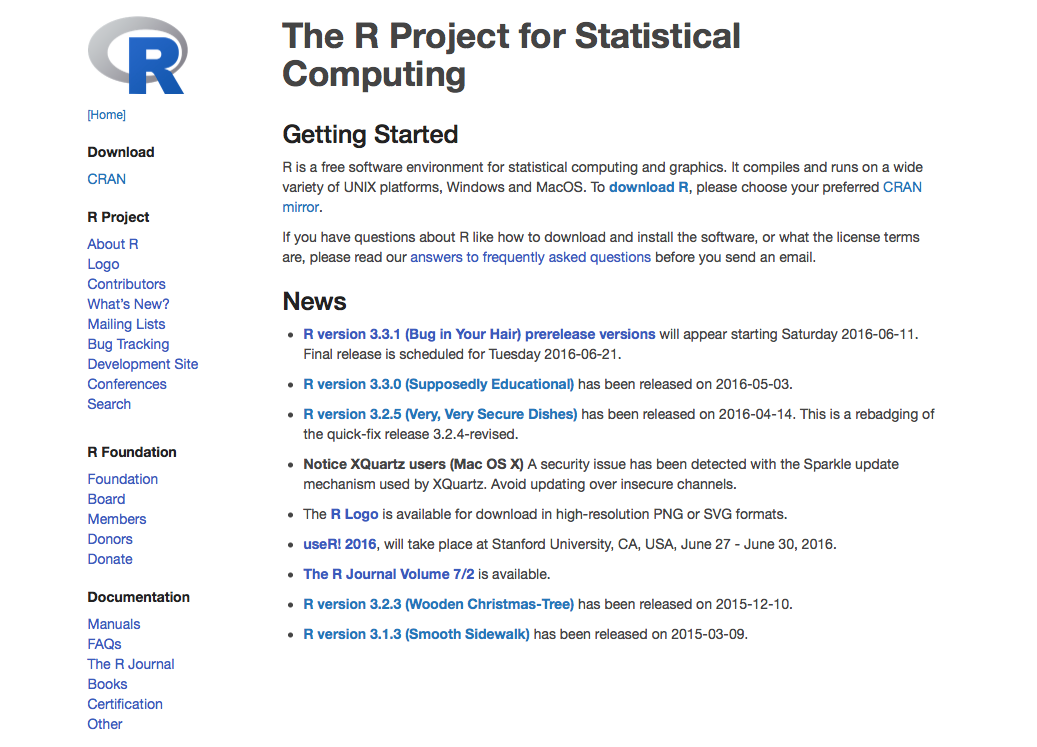
\includegraphics[scale=0.25]{figures/R-project.png}
\end{frame}

%%%%%%% 
\begin{frame}
	\frametitle{What R is?}
        \Large The \texttt{R} Project for Statistical Computing\\
	\begin{itemize}
		\small
		\item R version 3.3.1 (released 2016-06-21)
		\item Currently, the CRAN {\tiny(Comprehensive R Archive Network)} package repository features 8609 available packages
			\begin{itemize}
				\item \tiny \url{https://cran.r-project.org/web/packages/available_packages_by_name.html}
			\end{itemize}
		\item Currently, the Bioconductor repository features 1211 available packages
			\begin{itemize}
				\item \tiny \url{http://www.bioconductor.org}
			\end{itemize}
		\item Executed using command line, or a graphical user interface (GUI)
		\item On this course, we use the RStudio GUI
			\begin{itemize}
				\item \tiny \url{www.rstudio.com}
			\end{itemize}
	\end{itemize}
\end{frame}

%%%%%%% 
\begin{frame}[fragile]
	\frametitle{Getting started}
        \begin{itemize}
          \item \texttt{R} is a program which, once installed on your system, can be launched and is immediately ready to take input directly from the user\\
         
  \texttt{R} can be launched in 2 ways:
	  \begin{enumerate}
	    \item From command line
	      \begin{itemize}
		\item To start \texttt{R} you need to enter the console (also called terminal or shell)
		\item To start \texttt{R}, at the prompt simply type: \Large \texttt{R}
	      \end{itemize}
	    \item Using RStudio
	      \begin{itemize}
		  \item To launch RStudio, find the RStudio icon and double-click
		\end{itemize}
	    \end{enumerate}
  \end{itemize}
\end{frame}

%%%%%%% 
\begin{frame}
	\frametitle{RStudio}
	Since we will use RStudio in this course, let's have a look of the program\\
	\centering 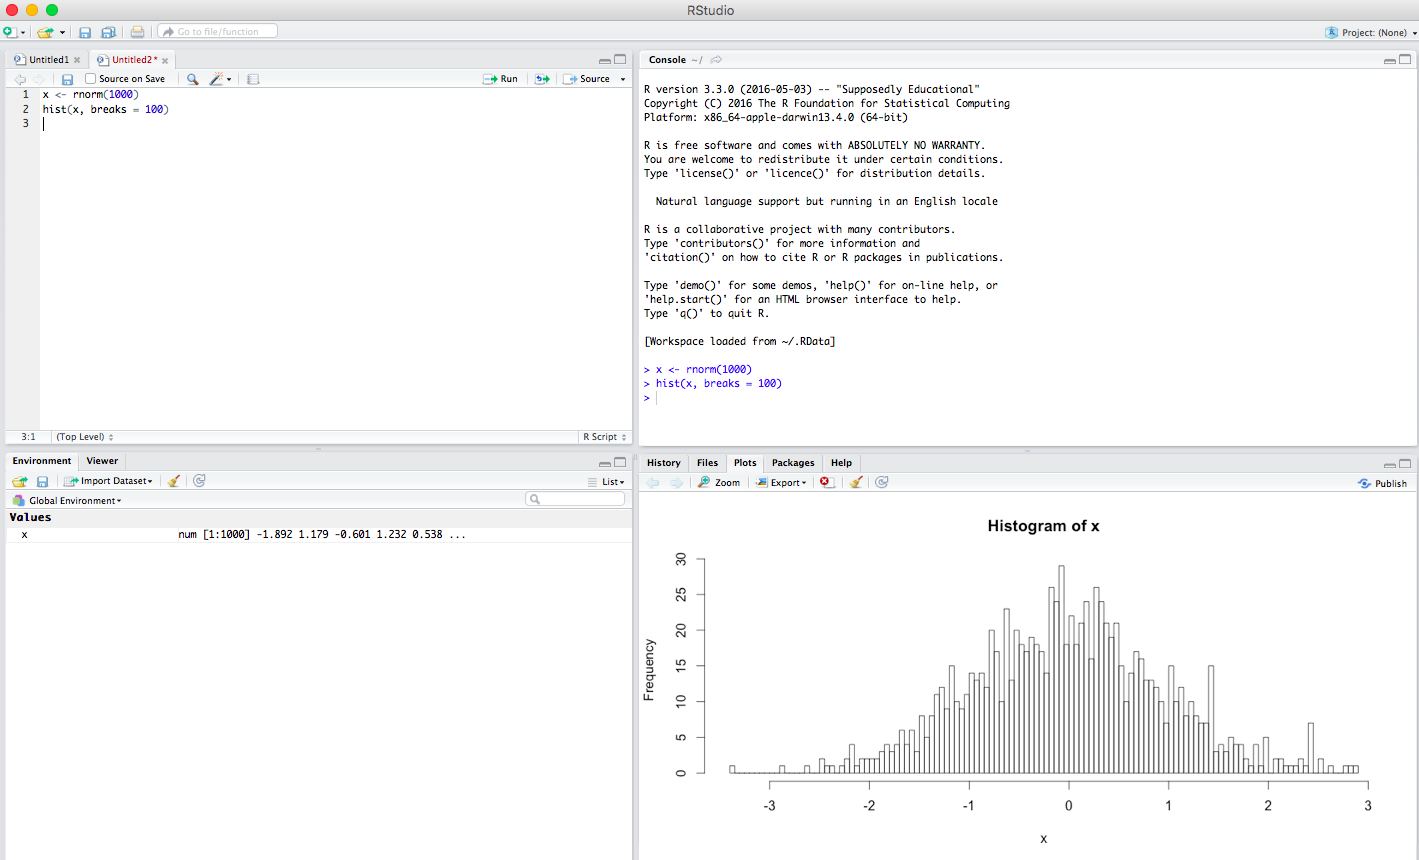
\includegraphics[scale=1.4]{figures/Rstudio_overview.png}
\end{frame}

%%%%%%% 
\begin{frame}
	\frametitle{RStudio}
	\textbf{R console}\\
	\vspace{20pt}
	\centering 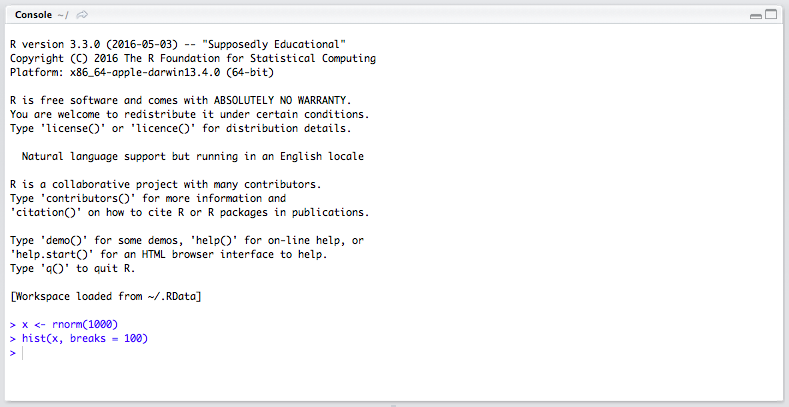
\includegraphics[width=11cm]{figures/RStudio_console.png}\\
	\small It is the place where you can interactively run R commands
\end{frame}

%%%%%%% 
\begin{frame}
	\frametitle{RStudio}
	\textbf{Source editor for R scripts}\\
	\vspace{20pt}
	\centering 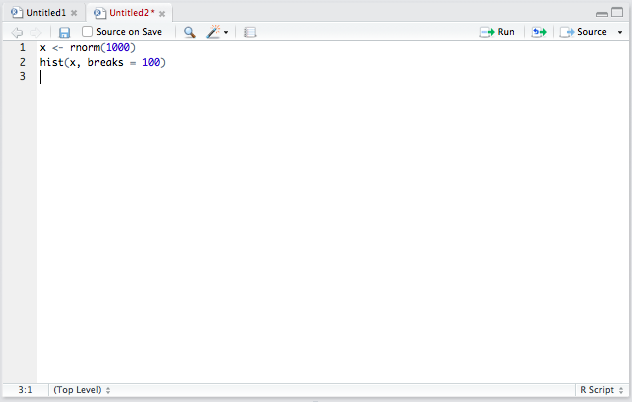
\includegraphics[width=10cm]{figures/RStudio_script.png}\\
	\small It is the place where you can write your scripts
\end{frame}

%%%%%%% 
\begin{frame}
	\frametitle{RStudio}
	\textbf{Workspace}\\
	\vspace{16pt}
	\centering 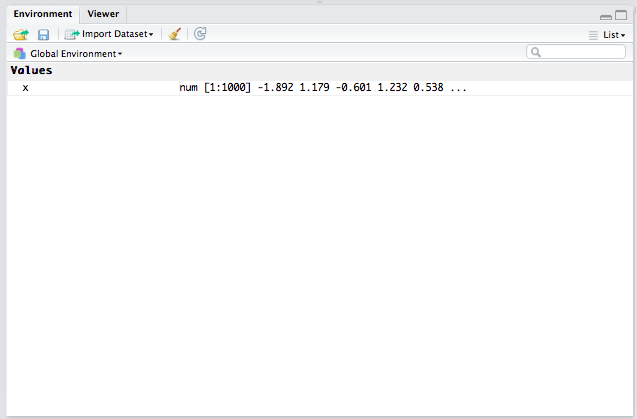
\includegraphics[width=10cm]{figures/RStudio_environment.png}\\
	\small It is the place where you can view object in the global environment
\end{frame}

%%%%%%% 
\begin{frame}
	\frametitle{RStudio}
	\textbf{Plot pannel}\\
	\vspace{20pt}
	\centering 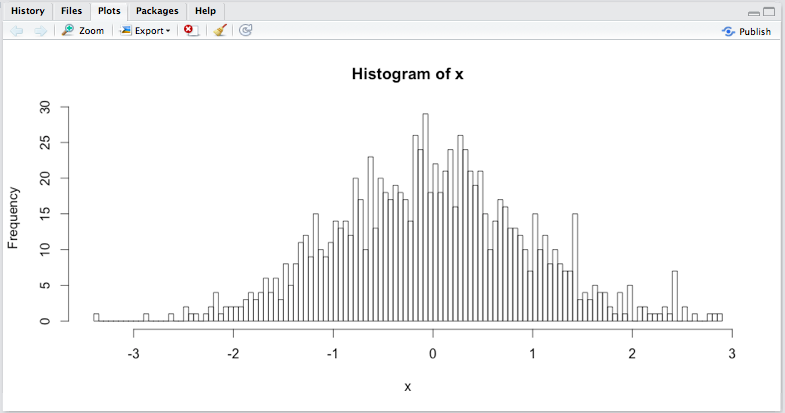
\includegraphics[width=10cm]{figures/RStudio_plot.png}\\
	\small It is the place where you can view your plots
\end{frame}

%%%%%%% 
\begin{frame}
	\frametitle{RStudio}
	\textbf{R help}\\
	\vspace{20pt}
	\centering 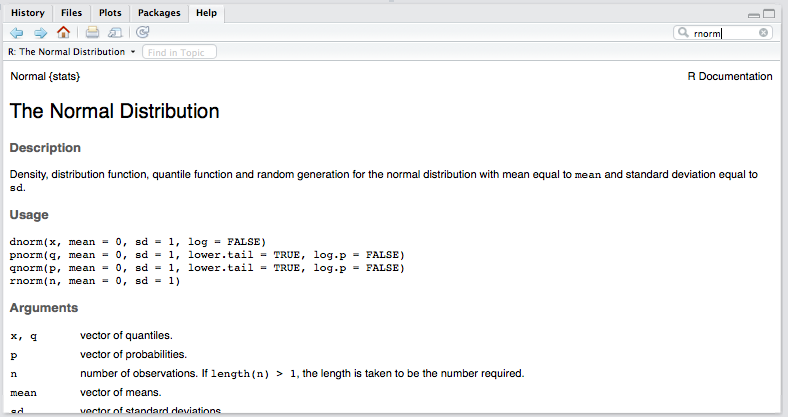
\includegraphics[width=10cm]{figures/RStudio_help.png}\\
	\small It is the place where you can find help
\end{frame}

%%%%%%% 
\begin{frame}
	\frametitle{RStudio}
	The GUI is divided into 4 main sub-windows\\
	These sub-windows are customizable\\
	\vspace{10pt}
	\centering 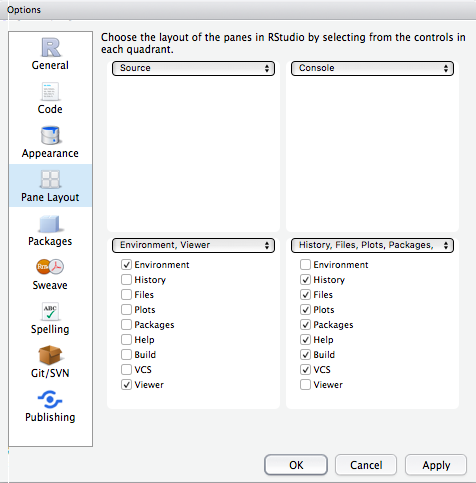
\includegraphics[width=7cm]{figures/RStudio_option.png}
\end{frame}

%%%%%%%%%%%%%%%%%%%%%%%%%%%%%%%%%%%%%%%%%%%%%%%%%%%%%%%%%%%%%%%%%%%%%%
%%%%%%%%%%%%%%%%%%%%%%%%%%%%%%%%%%%%%%%%%%%%%%%%%%%%%%%%%%%%%%%%%%%%%%
\begin{frame}
\section{Basic concepts in R}
\vspace{30pt}
\scriptsize
\begin{flushright}  Based on \url{https://github.com/lgatto/TeachingMaterial/tree/master/\_basicr} \end{flushright}
\end{frame}
%%%%%%% 
\begin{frame}[fragile]{prova}
	\frametitle{Numbers}
	The command line can be used as a calculator
\rule{\textwidth}{0.4pt}
\begin{Schunk}
\begin{Sinput}
> 5 + 7 
\end{Sinput}
\begin{Soutput}
[1] 12
\end{Soutput}
\begin{Sinput}
> 5 - 7
\end{Sinput}
\begin{Soutput}
[1] -2
\end{Soutput}
\begin{Sinput}
> 5 * 7
\end{Sinput}
\begin{Soutput}
[1] 35
\end{Soutput}
\begin{Sinput}
> 5 / 7
\end{Sinput}
\begin{Soutput}
[1] 0.7142857
\end{Soutput}
\end{Schunk}
\rule{\textwidth}{0.4pt}
\vspace{5pt}
\small Note: The number in the square brackets is an indicator of the position in the output
\end{frame}

%%%%%%% 
\begin{frame}[fragile]{prova}
	\frametitle{Numbers}
	You can solve simple or complex calculations 
	\rule{\textwidth}{0.4pt}
\begin{Schunk}
\begin{Sinput}
> (((20/5)^2)-((5+1/3+4/5-10)*(2-34))-20)
\end{Sinput}
\begin{Soutput}
[1] -127.7333
\end{Soutput}
\end{Schunk}
\rule{\textwidth}{0.4pt}
\vspace{20pt}
\Large But, of course, \texttt{R} is not a calculator
\end{frame}

%%%%%%% 
\begin{frame}[fragile]
	\frametitle{Variables}
	A \textbf{variable} is a letter or word which takes (or contains) a value. We use the assignment 'operator', <-\\
	\vspace{10pt}
	- We can assign a number to a variable
	\rule{\textwidth}{0.4pt}
\begin{Schunk}
\begin{Sinput}
> x <- 5
> x
\end{Sinput}
\begin{Soutput}
[1] 5
\end{Soutput}
\end{Schunk}
 \rule{\textwidth}{0.4pt}
 - We can assign the result of an operation to a variable
 \rule{\textwidth}{0.4pt}
\begin{Schunk}
\begin{Sinput}
> y <- 5 + 7
> y
\end{Sinput}
\begin{Soutput}
[1] 12
\end{Soutput}
\end{Schunk}
\rule{\textwidth}{0.4pt}
\end{frame}

%%%%%%% 
\begin{frame}[fragile]
	\frametitle{Variables}
	- We can assign use the variables to perform calculation
	\rule{\textwidth}{0.4pt}
\begin{Schunk}
\begin{Sinput}
> x + y
\end{Sinput}
\begin{Soutput}
[1] 17
\end{Soutput}
\end{Schunk}
 \rule{\textwidth}{0.4pt}
 - We can assign the change the content of the variable
 \rule{\textwidth}{0.4pt}
\begin{Schunk}
\begin{Sinput}
> x
\end{Sinput}
\begin{Soutput}
[1] 5
\end{Soutput}
\begin{Sinput}
> x <- x - y
> x
\end{Sinput}
\begin{Soutput}
[1] -7
\end{Soutput}
\end{Schunk}
\rule{\textwidth}{0.4pt}
\end{frame}

%%%%%%% 
\begin{frame}[fragile]
	\frametitle{Function}
	\textbf{Functions} in \texttt{R} perform operations on arguments (the input(s) to the function). \\ Arguments are always contained in parentheses, i.e. curved brackets (), separated by commas.
	\vspace{10pt}
	
\begin{Schunk}
\begin{Sinput}
> sum(3, 4, 5, 6)
\end{Sinput}
\begin{Soutput}
[1] 18
\end{Soutput}
\begin{Sinput}
> max(3, 4, 5, 6)
\end{Sinput}
\begin{Soutput}
[1] 6
\end{Soutput}
\begin{Sinput}
> min(3, 4, 5, 6)
\end{Sinput}
\begin{Soutput}
[1] 3
\end{Soutput}
\end{Schunk}

\end{frame}

%%%%%%% 
\begin{frame}[fragile]
	\frametitle{Function extention}
	\texttt{R} contains a lot of pre-builtin functions, but through the so called \textit{packages} is possible extend the \texttt{R} functionalities enormously.
	\vspace{30pt}
	Alternatevely, you can write your own function
\begin{Schunk}
\begin{Sinput}
> summ <- function(a,b){ a + b }
> summ(1,2)
\end{Sinput}
\begin{Soutput}
[1] 3
\end{Soutput}
\end{Schunk}
\end{frame}



\subsection{Vector}
%%%%%%% 
\begin{frame}
	\centering \Huge Vector
\end{frame}

%%%%%%% 
\begin{frame}[fragile]
	\frametitle{Vector}
	The basic data structure in \texttt{R} is a \textbf{vector}, an ordered collection of values. \texttt{R} even treats single values as 1-element vectors.\\
	The simplest way to create a \textbf{vector} in \texttt{R} is by using the c() operator:
	\rule{\textwidth}{0.4pt}
\begin{Schunk}
\begin{Sinput}
> c(1,2,3,50)
\end{Sinput}
\begin{Soutput}
[1]  1  2  3 50
\end{Soutput}
\end{Schunk}
\rule{\textwidth}{0.4pt}
\vspace{20pt}
\end{frame}

%%%%%%% 
\begin{frame}[fragile]
	\frametitle{Vector}
	The simplest way to create a \textbf{sequence of numbers} is by using the `:` operator:
	\rule{\textwidth}{0.4pt}
\begin{Schunk}
\begin{Sinput}
> 1:10
\end{Sinput}
\begin{Soutput}
 [1]  1  2  3  4  5  6  7  8  9 10
\end{Soutput}
\end{Schunk}
\rule{\textwidth}{0.4pt}
\vspace{20pt}
That gave us every integer between (and including) 1 and 10.
\end{frame}

%%%%%%% 
\begin{frame}[fragile]
	\frametitle{Vector}
	What happens if we do 15:1? Give it a try to find out.
	\pause
	\rule{\textwidth}{0.4pt}
\begin{Schunk}
\begin{Sinput}
> 15:1
\end{Sinput}
\begin{Soutput}
 [1] 15 14 13 12 11 10  9  8  7  6  5  4  3  2  1
\end{Soutput}
\end{Schunk}
\rule{\textwidth}{0.4pt}\\
\vspace{20pt}
It counted backwards in increments of 1!
\end{frame}

%%%%%%% 
\begin{frame}[fragile]
	\frametitle{Vector}
  	Remember that if you have questions about a particular R function, you can access its documentation with a question mark followed by the function name:\\
\begin{equation}?function name here \end{equation}\\
  However, in the case of an operator like the colon used above, you must enclose the symbol in backticks like this:\\
  \begin{equation}?`: \end{equation}\\
\end{frame}

%%%%%%% 
\begin{frame}[fragile]
	\frametitle{Vector}
	Often, we'll desire more control over a sequence we're creating than what the `:` operator gives us. The seq() function serves this purpose.\\
	\centering Try it: \small Remember what we said about the function arguments\\
	\pause
	\rule{\textwidth}{0.4pt}
\begin{Schunk}
\begin{Sinput}
> seq(1,10)
\end{Sinput}
\begin{Soutput}
 [1]  1  2  3  4  5  6  7  8  9 10
\end{Soutput}
\end{Schunk}
	\rule{\textwidth}{0.4pt}
\end{frame}

%%%%%%% 
\begin{frame}[fragile]
	\frametitle{Vector}
	This gives us the same output as 1:10. However, let's say that instead we want a vector of numbers ranging from 0 to 4, incremented by 0.5. seq(0, 4,by=0.5) does just that.\\
	\centering Try it out.\\
	\pause
	\rule{\textwidth}{0.4pt}
\begin{Schunk}
\begin{Sinput}
> seq(0, 4, by = 0.5)
\end{Sinput}
\begin{Soutput}
[1] 0.0 0.5 1.0 1.5 2.0 2.5 3.0 3.5 4.0
\end{Soutput}
\end{Schunk}
\rule{\textwidth}{0.4pt}
\end{frame}

%%%%%%% 
\begin{frame}[fragile]
	\frametitle{Vector}
	Or maybe we don't care what the increment is and we just want a sequence of 10 numbers between 5 and 10. seq(5, 10, length=10) does the trick. Give it a shot now and store the result in a new variable called \textit{mySeq}.\\
	\centering Try it out.\\
	\pause
\rule{\textwidth}{0.4pt}
\begin{Schunk}
\begin{Sinput}
> mySeq <- seq(5, 10, length=10)
> round(mySeq,1)
\end{Sinput}
\begin{Soutput}
 [1]  5.0  5.6  6.1  6.7  7.2  7.8  8.3  8.9  9.4 10.0
\end{Soutput}
\end{Schunk}
  \rule{\textwidth}{0.4pt}
\end{frame}

%%%%%%% 
\begin{frame}[fragile]
\frametitle{Vector}
To confirm that mySeq has length 10, we can use the length() function.\\
\centering Try it now\\
\pause
\rule{\textwidth}{0.4pt}
\begin{Schunk}
\begin{Sinput}
> length(mySeq)
\end{Sinput}
\begin{Soutput}
[1] 10
\end{Soutput}
\end{Schunk}
  \rule{\textwidth}{0.4pt}
\end{frame}

%%%%%%% 
\begin{frame}[fragile]
	\frametitle{Vector}
	\begin{itemize}
  	\item Let's pretend we don't know the length of mySeq, but we want to generate a sequence of integers from 1 to N, where N represents the length of the mySeq vector.
  	\item We want a new vector (1, 2, 3, ...) that is the same length as mySeq.
  	\item There are several ways we could do this. 
  	\item One possibility is to combine the `:` operator and the length() function.
	\end{itemize}
	\centering Give that a try
	\pause
\rule{\textwidth}{0.4pt}
\begin{Schunk}
\begin{Sinput}
> 1:length(mySeq)
\end{Sinput}
\begin{Soutput}
 [1]  1  2  3  4  5  6  7  8  9 10
\end{Soutput}
\end{Schunk}
\rule{\textwidth}{0.4pt}
\end{frame}

%%%%%%% 
\begin{frame}[fragile]
	\frametitle{Vector}
	Another option is to use seq(along.with = mySeq). Give that a try.
\rule{\textwidth}{0.4pt}
\begin{Schunk}
\begin{Sinput}
> seq(along.with = mySeq)
\end{Sinput}
\begin{Soutput}
 [1]  1  2  3  4  5  6  7  8  9 10
\end{Soutput}
\end{Schunk}
\rule{\textwidth}{0.4pt}\\
\vspace{20pt}
R has a separate built-in function for this purpose
\rule{\textwidth}{0.4pt}
\begin{Schunk}
\begin{Sinput}
> seq_along(mySeq)
\end{Sinput}
\begin{Soutput}
 [1]  1  2  3  4  5  6  7  8  9 10
\end{Soutput}
\end{Schunk}
\rule{\textwidth}{0.4pt}
\end{frame}

%%%%%%% 
\begin{frame}[fragile]
	\frametitle{Vector}
	\begin{itemize}
	\item There are often \textbf{several approaches} to solving the same problem in \texttt{R}          \item Simple approaches that involve \textbf{less typing} are generally best
	\item It is also important for your code to be \textbf{readable}, so that you and others can figure out what's going on without too much hassle
	\end{itemize}
\rule{\textwidth}{0.4pt}
\begin{Schunk}
\begin{Sinput}
> # Create a sequence of 10 numbers
> seq_along(mySeq)
\end{Sinput}
\begin{Soutput}
 [1]  1  2  3  4  5  6  7  8  9 10
\end{Soutput}
\end{Schunk}
\rule{\textwidth}{0.4pt}
\small The comments in \texttt{R} begin with \textbf{hash}. You should have about 1/3 of your code commented. 
\end{frame}

%%%%%%% 
\begin{frame}[fragile]
	\frametitle{Vector}
	One more function related to creating sequences of numbers is rep(), which stands for 'replicate'.\\
	If we're interested in creating a vector that contains 1 and 0 five times, we can use rep(c(1,0), times = 5).\\
	\centering Try it out
	\pause
	\rule{\textwidth}{0.4pt}
\begin{Schunk}
\begin{Sinput}
> # Create a sequence of 1 and 0
> rep(c(1,0), times = 5)
\end{Sinput}
\begin{Soutput}
 [1] 1 0 1 0 1 0 1 0 1 0
\end{Soutput}
\end{Schunk}
\rule{\textwidth}{0.4pt}
\end{frame}

%%%%%%% 
\begin{frame}[fragile]
	\frametitle{Vector}
If we want our vector to contain 5 ones and then 5 zeros, we can do this with the `each` argument instead of `times` argument.\\
  \centering Try it out\\
  \pause
  \rule{\textwidth}{0.4pt}
\begin{Schunk}
\begin{Sinput}
> # Create a sequence of 1 and 0
> rep(c(1,0), each = 5)
\end{Sinput}
\begin{Soutput}
 [1] 1 1 1 1 1 0 0 0 0 0
\end{Soutput}
\end{Schunk}
\rule{\textwidth}{0.4pt}
\end{frame}

%%%%%%% 
\begin{frame}[fragile]
	\frametitle{Vector}
	\begin{itemize}
	\item We'll see, now, how to \textbf{extract} elements from a vector (subset)
	\item The square brackets \textbf{[]} indicate position within the vector
	  \begin{itemize}
	    \small
	    \item \texttt{R} even treats single values as 1-element vectors
	    \item The vector in \texttt{R} starts from position 1
	  \end{itemize}
	\item We can extract individual elements by using the \textbf{[]} notation
  \end{itemize}
  \centering Try mySeq[1:3]\\
  \pause
  \rule{\textwidth}{0.4pt}
\begin{Schunk}
\begin{Sinput}
> mySeq[1:3]
\end{Sinput}
\begin{Soutput}
[1] 5.000000 5.555556 6.111111
\end{Soutput}
\end{Schunk}
\rule{\textwidth}{0.4pt}
\end{frame}

%%%%%%% 
\begin{frame}[fragile]
	\frametitle{Vector}
	If we want to 3th, 5th and 10th elements of the vector mySeq.\\
	\centering Try it out
	\pause
	\rule{\textwidth}{0.4pt}
\begin{Schunk}
\begin{Sinput}
> round(mySeq,1)
\end{Sinput}
\begin{Soutput}
 [1]  5.0  5.6  6.1  6.7  7.2  7.8  8.3  8.9  9.4 10.0
\end{Soutput}
\begin{Sinput}
> round(mySeq[c(3,5,10)],1)
\end{Sinput}
\begin{Soutput}
[1]  6.1  7.2 10.0
\end{Soutput}
\end{Schunk}
  \rule{\textwidth}{0.4pt}
\end{frame}

%%%%%%% 
\begin{frame}[fragile]
	\frametitle{Vector}
	If we want all the elements bigger than 7.\\
	\centering Try it out\\
	\pause
		\rule{\textwidth}{0.4pt}
\begin{Schunk}
\begin{Sinput}
> round(mySeq,1)
\end{Sinput}
\begin{Soutput}
 [1]  5.0  5.6  6.1  6.7  7.2  7.8  8.3  8.9  9.4 10.0
\end{Soutput}
\begin{Sinput}
> round(mySeq[mySeq > 7],1)
\end{Sinput}
\begin{Soutput}
[1]  7.2  7.8  8.3  8.9  9.4 10.0
\end{Soutput}
\end{Schunk}
  \rule{\textwidth}{0.4pt}
\end{frame}

%%%%%%% 
\begin{frame}[fragile]
	\frametitle{Vector}
	If we ask you to produce a vector of 1000 even numbers (from 2 to 2000), extract the 345th and the 987th elements and sum them, would you know how to do it?\\
	\centering Try it out
	\pause
		\rule{\textwidth}{0.4pt}
\begin{Schunk}
\begin{Sinput}
> a <- seq(2,2000,by=2)
> length(a)
\end{Sinput}
\begin{Soutput}
[1] 1000
\end{Soutput}
\begin{Sinput}
> a[345] + a[987]
\end{Sinput}
\begin{Soutput}
[1] 2664
\end{Soutput}
\begin{Sinput}
> # Short version
> sum(seq(2,2000,by=2)[c(345,987)])
\end{Sinput}
\begin{Soutput}
[1] 2664
\end{Soutput}
\end{Schunk}
  \rule{\textwidth}{0.4pt}
\end{frame}

%%%%%%% 
\begin{frame}[fragile]
	\frametitle{Vector}
	When applying all standard arithmetic operations to vectors, \textbf{application is element-wise}.\\
\rule{\textwidth}{0.4pt}
\begin{Schunk}
\begin{Sinput}
> x <- 1:10
> y <- x * 2
> y
\end{Sinput}
\begin{Soutput}
 [1]  2  4  6  8 10 12 14 16 18 20
\end{Soutput}
\end{Schunk}
  \rule{\textwidth}{0.4pt}
\end{frame}


%%%%%%% 
\begin{frame}[fragile]
	\frametitle{Vector}
	Adding two vectors\\
\rule{\textwidth}{0.4pt}
\begin{Schunk}
\begin{Sinput}
> z <- x^2
> y + z
\end{Sinput}
\begin{Soutput}
 [1]   3   8  15  24  35  48  63  80  99 120
\end{Soutput}
\end{Schunk}
  \rule{\textwidth}{0.4pt}\\
  \vspace{20pt}
  If vectors are not the same length, the shorter one will be recycled\\
  \rule{\textwidth}{0.4pt}
\begin{Schunk}
\begin{Sinput}
> x
\end{Sinput}
\begin{Soutput}
 [1]  1  2  3  4  5  6  7  8  9 10
\end{Soutput}
\begin{Sinput}
> x + 1:2
\end{Sinput}
\begin{Soutput}
 [1]  2  4  4  6  6  8  8 10 10 12
\end{Soutput}
\end{Schunk}
  \rule{\textwidth}{0.4pt}
\end{frame}

%%%%%%% 
\begin{frame}[fragile]
	\frametitle{Vector}
	\begin{itemize}
	  \item All the vectors we have seen so far have contained numbers, but we can also store strings 
\rule{\textwidth}{0.4pt}
\footnotesize
\begin{Schunk}
\begin{Sinput}
> gene.names <- c("Pax6","Beta-actin","FoxP2","Hox9")
> gene.names
\end{Sinput}
\begin{Soutput}
[1] "Pax6"       "Beta-actin" "FoxP2"      "Hox9"      
\end{Soutput}
\end{Schunk}
  \rule{\textwidth}{0.4pt}\\
  \vspace{20pt}
  \normalsize
	  \item We can name elements of vectors using the \textit{names} function
\rule{\textwidth}{0.4pt}
\footnotesize
\begin{Schunk}
\begin{Sinput}
> gene.expression <- c(0,3.2,1.2,-2)
> gene.expression
\end{Sinput}
\begin{Soutput}
[1]  0.0  3.2  1.2 -2.0
\end{Soutput}
\begin{Sinput}
> names(gene.expression)<-gene.names
> gene.expression
\end{Sinput}
\begin{Soutput}
      Pax6 Beta-actin      FoxP2       Hox9 
       0.0        3.2        1.2       -2.0 
\end{Soutput}
\end{Schunk}
  \rule{\textwidth}{0.4pt}\\
  \normalsize
	\end{itemize}
	
\end{frame}

%%%%%%% 
\begin{frame}[fragile]
	\frametitle{Vector}
	\Large Exercise: genes and genomes
	\begin{itemize}
	\small
	  \item Let's try some \textbf{vector arithmetic}. Here are the genome lengths and number of protein coding genes for several model organisms:
	  \begin{table}[]
	  \scriptsize
\centering
\begin{tabular}{|l|c|c|}
\hline
\multicolumn{1}{|c|}{Species}     & Genome size (Mb) & Protein coding genes \\ \hline
\textit{Homo sapiens}             & 3,102            & 20,774               \\ \hline
\textit{Mus musculus}             & 2,731            & 23,139               \\ \hline
\textit{Drosophila melanogaster}  & 169              & 13,937               \\ \hline
\textit{Caenorhabditis elegans}   & 100              & 20,532               \\ \hline
\textit{Saccharomyces cerevisiae} & 12               & 6,692                \\ \hline
\end{tabular}
\end{table}
  \item Create \textbf{genome.size} and \textbf{coding.genes} vectors to hold the data in each column using the c function
  \item Create a \textbf{species.name} vector and use this vector to name the values in the other two vectors.
	\end{itemize}
\end{frame}

%%%%%%% 
\begin{frame}[fragile]
	\frametitle{Vector}
	\Large Exercise: genes and genomes
	\begin{itemize}
	\small
	  \item Let's assume a \textbf{coding gene has an average length of 1.5 kilobases} \footnotesize (1.5 kilobases is 0.0015 Megabases)
	  \small
	  \item On average, how many base pairs of each genome is made of coding genes? 
	  \item \textbf{Create a new vector to record this} called \textbf{coding.bases}
	  \item \textbf{What percentage of each genome is made up of protein coding genes?} 
	  \item Use your \textbf{coding.bases} and \textbf{genome.size} vectors to calculate this
	  \item \textbf{How many times more bases are used for coding in the human genome compared to the yeast genome?
	  \item How many times more bases are in the human genome in total compared to the yeast genome?}
	  \item Look up indices of your vectors to find out.
	 \end{itemize}
\end{frame}

%%%%%%% 
\begin{frame}[fragile]
	\frametitle{Vector}
	\Large Exercise: genes and genomes
	\begin{itemize}
	\small
	  \item Creating vectors:
\rule{\textwidth}{0.4pt}
\footnotesize
\begin{Schunk}
\begin{Sinput}
> genome.size<-c(3102,2731,169,100,12)
> coding.genes<-c(20774,23139,13937,20532,6692)
> species.name<-c("H. sapiens","M. musculus","D. melanogaster","C. elegans","S.
+ cerevisiae")
> names(genome.size)<-species.name
> names(coding.genes)<-species.name
\end{Sinput}
\end{Schunk}
  \rule{\textwidth}{0.4pt}\\
  \small
  \pause
    \item To calculate the number of coding bases, we need to use the same scale as we used for genome size: 1.5 kilobases is 0.0015 Megabases
\rule{\textwidth}{0.4pt}
\footnotesize
\begin{Schunk}
\begin{Sinput}
> coding.bases<-coding.genes*0.0015
> coding.bases
\end{Sinput}
\begin{Soutput}
     H. sapiens     M. musculus D. melanogaster      C. elegans  S.\ncerevisiae 
        31.1610         34.7085         20.9055         30.7980         10.0380 
\end{Soutput}
\end{Schunk}
  \rule{\textwidth}{0.4pt}\\
	\end{itemize}
\end{frame}

%%%%%%% 
\begin{frame}[fragile]
	\frametitle{Vector}
	\Large Exercise: genes and genomes
	\begin{itemize}
	\small
	  \item To calculate the percentage of coding bases in each genome:
\rule{\textwidth}{0.4pt}
\footnotesize
\begin{Schunk}
\begin{Sinput}
> coding.pc<-coding.bases/genome.size*100
> coding.pc
\end{Sinput}
\begin{Soutput}
     H. sapiens     M. musculus D. melanogaster      C. elegans  S.\ncerevisiae 
       1.004545        1.270908       12.370118       30.798000       83.650000 
\end{Soutput}
\end{Schunk}
  \rule{\textwidth}{0.4pt}\\
  \small
  \pause
    \item To compare human to yeast:
\rule{\textwidth}{0.4pt}
\footnotesize
\begin{Schunk}
\begin{Sinput}
> coding.bases[1]/coding.bases[5]
\end{Sinput}
\begin{Soutput}
H. sapiens 
  3.104304 
\end{Soutput}
\begin{Sinput}
> genome.size[1]/genome.size[5]
\end{Sinput}
\begin{Soutput}
H. sapiens 
     258.5 
\end{Soutput}
\end{Schunk}
  \rule{\textwidth}{0.4pt}\\
	\end{itemize}
\end{frame}

%%%%%%% 
\begin{frame}[fragile]
	\frametitle{Vector}
	\Large Exercise: genes and genomes
	\begin{itemize}
	\small
	  \item Note that if a new vector is created using a named vector, the names are usually carried across to the new vector. Sometimes this is what we want (as for \textbf{coding.pc}) but sometimes it is not (when we are comparing human to yeast). We can remove names by setting them to the special NULL value:
\rule{\textwidth}{0.4pt}
\footnotesize
\begin{Schunk}
\begin{Sinput}
> names(coding.pc)<-NULL
> coding.pc
\end{Sinput}
\begin{Soutput}
[1]  1.004545  1.270908 12.370118 30.798000 83.650000
\end{Soutput}
\end{Schunk}
  \rule{\textwidth}{0.4pt}\\
	\end{itemize}
\end{frame}

\subsection{R packages}
\begin{frame}
	\centering \Huge R packages
\end{frame}

\begin{frame}[fragile]
	\frametitle{R packages}
	\begin{itemize}
	\small
\item \texttt{R} comes ready loaded with various libraries of functions called \textbf{packages}. e.g. the function \textbf{sum()} is in the base package and \textbf{sd()}, which calculates the standard deviation of a vector, is in the stats package
	\pause
		\item There are 1000s of additional packages provided by third parties, and the packages can be found in numerous server locations on the web called repositories
	\pause
		\item The two repositories you will come across the most are
			\begin{itemize}
				\item The Comprehensive R Archive Network (CRAN)
				\item Bioconductor
			\end{itemize}
	\pause
		\item CRAN is mirrored in many locations. Set your local mirror in RStudio using Tools > Options, and choose a CRAN mirror
	\pause
		\item Bioconductor packages are then loaded with the biocLite() function
			\begin{itemize}
				\item source(``http://bioconductor.org/biocLite.R'')
				\item biocLite(``PackageName'')
			\end{itemize}
	\end{itemize}
\end{frame}

 
\begin{frame}[fragile]
	\frametitle{R package}
	\centering \Huge Exercise
	\begin{itemize}
	\small
		\item Matrix is a CRAN extras packageUse
			\begin{itemize}
				\item Use \textbf{install.packages()} function\ldots
			%	\item install.packages(``Matrix'')
				\item or in RStudio goto Tools > Install Packages\ldots and type the package name
			\end{itemize}
		\item aCGH is a BioConductor package (www.bioconductor.org)
		%	\begin{itemize}
			%	\item source(``http://bioconductor.org/biocLite.R'') 
			%	\item biocLite(``aCGH'')
		%	\end{itemize}
	\end{itemize}
\end{frame}

\begin{frame}[fragile]
	\frametitle{R package}
	\begin{itemize}
	\small
		\item \texttt{R} needs to be told to use the new functions from the installed packages 
		\item Use \textbf{library(\ldots)} function to load the newly installed features
		\item \textbf{library(``Matrix'')};  loads matrix functions
	\end{itemize}
	\footnotesize PS: Library(): Lists all the packages you've got installed locally
\end{frame}


\subsection{Data structures}


%%%%%%% 
\begin{frame}[fragile]
	\frametitle{Data structures}
	\centering \LARGE \texttt{R} is designed to handle experimental data
	\begin{itemize}
		\small
		\item In this lesson, we'll cover \textbf{matrices} and \textbf{data frames}. Both represent 'rectangular' data types, meaning that they are used to store tabular data, with rows and columns
		\item The main difference, as you'll see, is that \textbf{matrices} can only contain a single class of data, while \textbf{data frames} can consist of many different classes of data
	\end{itemize}
\end{frame}

%%%%%%% 
\begin{frame}[fragile]
	\frametitle{Data frame}
	\begin{itemize}
		\small
		\item A data frame is a \textbf{set of observations} of a set of variables  in other words, the \underline{outcome of an experiment}.\\ 
			\tiny [Wickham, H. (2014). Tidy Data. Journal of Statistical Software, 59(10), 1 - 23] 

		\small
		\item For example, we might want to analyse information about a set of patients. To start with, let's say we have ten patients and for each one we know their \textbf{name, sex, age, weight and whether they give consent} for their data to be made public
		\item We are going to create a data frame called 'patients', which will have \underline{ten rows (observations)} and \underline{seven columns (variables)}. 
		\item \textbf{The columns must all be equal lengths}

	\end{itemize}
\end{frame}

%%%%%%% 
\begin{frame}[fragile]
	\frametitle{Data frame}
	\centering \LARGE The patients data frame
	\vspace{20pt}
\tiny
\begin{Schunk}
\begin{Sinput}
> patients
\end{Sinput}
\begin{Soutput}
   firstName secondName paste.firstName..secondName.    sex age weight consent
1       Adam      Jones                   Adam Jones   Male  50   70.8    TRUE
2        Eve     Parker                   Eve Parker Female  21   67.9    TRUE
3       John      Evans                   John Evans   Male  35   75.3   FALSE
4       Mary      Davis                   Mary Davis Female  45   61.9    TRUE
5      Peter      Baker                  Peter Baker   Male  28   72.4   FALSE
6       Paul    Daniels                 Paul Daniels   Male  31   69.9   FALSE
7     Joanna    Edwards               Joanna Edwards Female  42   63.5   FALSE
8    Matthew      Smith                Matthew Smith   Male  33   71.5    TRUE
9      David    Roberts                David Roberts   Male  57   73.2   FALSE
10     Sally     Wilson                 Sally Wilson Female  62   64.8    TRUE
\end{Soutput}
\end{Schunk}
\small
\end{frame}

%%%%%%% 
\begin{frame}[fragile]
	\frametitle{Data frame}
	\begin{itemize}
		\small
		\item \textbf{Each column is a vector}, like previous vectors we have seen, for example:
\rule{\textwidth}{0.4pt}
\scriptsize
\begin{Schunk}
\begin{Sinput}
> age<-c(50, 21, 35, 45, 28, 31, 42, 33, 57, 62)
> weight<-c(70.8, 67.9, 75.3, 61.9, 72.4, 69.9, 63.5, 71.5, 73.2, 64.8)
\end{Sinput}
\end{Schunk}
\rule{\textwidth}{0.4pt}\\
\small
\vspace{10pt}
		\item We can define the names using character vectors:
\rule{\textwidth}{0.4pt}
\scriptsize
\begin{Schunk}
\begin{Sinput}
> firstName<-c('Adam', 'Eve', 'John', 'Mary', 'Peter', 'Paul', 
+ 	     'Joanna','Matthew', 'David', 'Sally')
> secondName<-c('Jones', 'Parker', 'Evans', 'Davis', 'Baker', 
+ 	       'Daniels', 'Edwards', 'Smith', 'Roberts', 'Wilson')
\end{Sinput}
\end{Schunk}
\rule{\textwidth}{0.4pt}\\
\small
\vspace{10pt}
		\item We also have a new type of vector, the logical vector, which only contains the values TRUE and FALSE:
\rule{\textwidth}{0.4pt}
\scriptsize
\begin{Schunk}
\begin{Sinput}
> consent<-c(TRUE,TRUE,FALSE,TRUE,FALSE,FALSE,FALSE,TRUE,FALSE,TRUE)
\end{Sinput}
\end{Schunk}
\rule{\textwidth}{0.4pt}\\\end{itemize}
\end{frame}


%%%%%%% 
\begin{frame}[fragile]
	\frametitle{Data structures}
	\begin{itemize}
		\small
		\item \textbf{Vectors can only contain one type of data}; we cannot mix numbers, characters and logical values in the same vector 
		\item If we try this, R will convert everything to characters:
\rule{\textwidth}{0.4pt}
\scriptsize
\begin{Schunk}
\begin{Sinput}
> c(20, 'a string', TRUE)
\end{Sinput}
\begin{Soutput}
[1] "20"       "a string" "TRUE"    
\end{Soutput}
\end{Schunk}
\rule{\textwidth}{0.4pt}\\
\small
\vspace{10pt}
		\item We can see the type of a particular vector using the mode function
\rule{\textwidth}{0.4pt}
\footnotesize
\setlength{\fancyvrbtopsep}{-1pt}
\setlength{\fancyvrbpartopsep}{-1pt}
\begin{Schunk}
\begin{Sinput}
> mode(firstName)
\end{Sinput}
\begin{Soutput}
[1] "character"
\end{Soutput}
\begin{Sinput}
> mode(age)
\end{Sinput}
\begin{Soutput}
[1] "numeric"
\end{Soutput}
\begin{Sinput}
> mode(weight)
\end{Sinput}
\begin{Soutput}
[1] "numeric"
\end{Soutput}
\begin{Sinput}
> mode(consent)
\end{Sinput}
\begin{Soutput}
[1] "logical"
\end{Soutput}
\end{Schunk}
\rule{\textwidth}{0.4pt}\\
		\small
\vspace{10pt}
	\end{itemize}
\end{frame}


%%%%%%% 
\begin{frame}[fragile]
	\frametitle{Data structures}
	\begin{itemize}
		\small
		\item Character vectors are fine for some variables, like names
		\item But sometimes we have categorical data and we want \texttt{R} to recognize this
		\item \textbf{A factor is \texttt{R}'s data structure for categorical data}
\rule{\textwidth}{0.4pt}
\scriptsize
\setlength{\fancyvrbtopsep}{-1pt}
\setlength{\fancyvrbpartopsep}{-1pt}
\begin{Schunk}
\begin{Sinput}
> sex
\end{Sinput}
\begin{Soutput}
 [1] "Male"   "Female" "Male"   "Female" "Male"   "Male"   "Female" "Male"  
 [9] "Male"   "Female"
\end{Soutput}
\begin{Sinput}
> factor(sex)
\end{Sinput}
\begin{Soutput}
 [1] Male   Female Male   Female Male   Male   Female Male   Male   Female
Levels: Female Male
\end{Soutput}
\end{Schunk}
\rule{\textwidth}{0.4pt}\\
\small
\vspace{10pt}
		\item \texttt{R} has converted the strings of the sex character vector into two levels, which are the categories in the data
		\item Note the values of this factor are not character strings, but \texttt{levels}
		\item We can use this factor to compare data for males and females
	\end{itemize}
\end{frame}


%%%%%%% 
\begin{frame}[fragile]
	\frametitle{Data structures}
	\centering \LARGE Creating a data frame
	\begin{itemize}
		\small
		\item We can construct a data frame from other objects
\rule{\textwidth}{0.4pt}
\tiny
\begin{Schunk}
\begin{Sinput}
> patients<-data.frame(firstName, secondName, paste(firstName,secondName),
+ 		     sex, age, weight, consent)
> patients
\end{Sinput}
\begin{Soutput}
   firstName secondName paste.firstName..secondName.    sex age weight consent
1       Adam      Jones                   Adam Jones   Male  50   70.8    TRUE
2        Eve     Parker                   Eve Parker Female  21   67.9    TRUE
3       John      Evans                   John Evans   Male  35   75.3   FALSE
4       Mary      Davis                   Mary Davis Female  45   61.9    TRUE
5      Peter      Baker                  Peter Baker   Male  28   72.4   FALSE
6       Paul    Daniels                 Paul Daniels   Male  31   69.9   FALSE
7     Joanna    Edwards               Joanna Edwards Female  42   63.5   FALSE
8    Matthew      Smith                Matthew Smith   Male  33   71.5    TRUE
9      David    Roberts                David Roberts   Male  57   73.2   FALSE
10     Sally     Wilson                 Sally Wilson Female  62   64.8    TRUE
\end{Soutput}
\end{Schunk}
\rule{\textwidth}{0.4pt}\\
\small
		\item The paste function joins character vectors together
		\item We can access particular variables using the dollar operator
\rule{\textwidth}{0.4pt}
\tiny
\begin{Schunk}
\begin{Sinput}
> patients$age
\end{Sinput}
\begin{Soutput}
 [1] 50 21 35 45 28 31 42 33 57 62
\end{Soutput}
\end{Schunk}
\rule{\textwidth}{0.4pt}\\
\small
	\end{itemize}
\end{frame}

%%%%%%% 
\begin{frame}[fragile]
	\frametitle{Data structures}
	\centering \LARGE Naming data frame variables
	\begin{itemize}
		\small
		\item \texttt{R} has inferred the names of our data frame variables from the names of the vectors or the commands (eg the paste command)
		\item We can name the variables after we have created a data frame using the \textbf{names} function, and we can use the same function to see the names
\rule{\textwidth}{0.4pt}
\tiny
\begin{Schunk}
\begin{Sinput}
> names(patients)<-c('First_Name', 'Second_Name', 'Full_Name', 'Sex',
+ 		   'Age', 'Weight', 'Consent')
> names(patients)
\end{Sinput}
\begin{Soutput}
[1] "First_Name"  "Second_Name" "Full_Name"   "Sex"         "Age"        
[6] "Weight"      "Consent"    
\end{Soutput}
\end{Schunk}
\rule{\textwidth}{0.4pt}\\
\vspace{10pt}
\small
		\item Or we can name the variables when we define the data frame
\rule{\textwidth}{0.4pt}
\tiny
\begin{Schunk}
\begin{Sinput}
> patients<-data.frame(First_Name=firstName, Second_Name=secondName,
+ 		     Full_Name=paste(firstName,secondName), Sex=sex,
+ 		     Age=age, Weight=weight, Consent=consent)
> names(patients)
\end{Sinput}
\begin{Soutput}
[1] "First_Name"  "Second_Name" "Full_Name"   "Sex"         "Age"        
[6] "Weight"      "Consent"    
\end{Soutput}
\end{Schunk}
\rule{\textwidth}{0.4pt}\\
\small
	\end{itemize}
\end{frame}

%%%%%%% 
\begin{frame}[fragile]
	\frametitle{Data structures}
	\centering \LARGE Matrices
	\begin{itemize}
		\small
	\item Data frames are \texttt{R} speciality, but R also handles matrices
\rule{\textwidth}{0.4pt}
\tiny
\begin{Schunk}
\begin{Sinput}
> e <- matrix(1:10, nrow=5, ncol=2)
> e
\end{Sinput}
\begin{Soutput}
     [,1] [,2]
[1,]    1    6
[2,]    2    7
[3,]    3    8
[4,]    4    9
[5,]    5   10
\end{Soutput}
\end{Schunk}
\vspace{20pt}
\begin{Schunk}
\begin{Sinput}
> f <-  matrix(1:10, nrow=2, ncol=5)
> f
\end{Sinput}
\begin{Soutput}
     [,1] [,2] [,3] [,4] [,5]
[1,]    1    3    5    7    9
[2,]    2    4    6    8   10
\end{Soutput}
\end{Schunk}
\rule{\textwidth}{0.4pt}\\
\small
	\end{itemize}
\end{frame}



%%%%%%% 
\begin{frame}[fragile]
	\frametitle{Data structures}
	\centering \LARGE Lists
	\begin{itemize}
		\small
		\item We have seen that vectors can only hold data of one type. 
		\item \underline{How can we store data of multiple types?} 
		\item \underline{Or vectors of different lengths in one object?}
		\item We can use lists; a list can contain \textbf{objects of any type}
\rule{\textwidth}{0.4pt}
\tiny
\begin{Schunk}
\begin{Sinput}
> a <- 1:10
> b <- matrix(runif(100),ncol=10,nrow=10)
> c <- data.frame(a, month.name[1:10])
> myList<-list( ls.obj.1=a, ls.obj.2=b,ls.obj.3=c )
> summary(myList)
\end{Sinput}
\begin{Soutput}
         Length Class      Mode   
ls.obj.1  10    -none-     numeric
ls.obj.2 100    -none-     numeric
ls.obj.3   2    data.frame list   
\end{Soutput}
\end{Schunk}
\vspace{20pt}
\setlength{\fancyvrbtopsep}{-1pt}
\setlength{\fancyvrbpartopsep}{-1pt}
\begin{Schunk}
\begin{Sinput}
> names(myList)
\end{Sinput}
\begin{Soutput}
[1] "ls.obj.1" "ls.obj.2" "ls.obj.3"
\end{Soutput}
\end{Schunk}

\rule{\textwidth}{0.4pt}\\
\small
	\end{itemize}
\end{frame}


%%%%%%% 
\begin{frame}[fragile]
	\frametitle{Data structures}
	\centering \LARGE Indexing data frames and matrices
	\begin{itemize}
		\small
		\item You can index multidimensional data structures like:\\ \Large \textbf{object [ rows , columns ]}
		\small
		\item If you don't provide an index for either rows or columns, all of the rows or columns will be returned
\rule{\textwidth}{0.4pt}
\tiny
\setlength{\fancyvrbtopsep}{-1pt}
\setlength{\fancyvrbpartopsep}{-1pt}
\begin{Schunk}
\begin{Sinput}
> patients[1,2]
\end{Sinput}
\begin{Soutput}
[1] Jones
10 Levels: Baker Daniels Davis Edwards Evans Jones Parker Roberts ... Wilson
\end{Soutput}
\end{Schunk}
\vspace{20pt}
\setlength{\fancyvrbtopsep}{-1pt}
\setlength{\fancyvrbpartopsep}{-1pt}
\begin{Schunk}
\begin{Sinput}
> patients[1,]
\end{Sinput}
\begin{Soutput}
  First_Name Second_Name  Full_Name  Sex Age Weight Consent
1       Adam       Jones Adam Jones Male  50   70.8    TRUE
\end{Soutput}
\end{Schunk}
\vspace{20pt}
\begin{Schunk}
\begin{Sinput}
> patients[patients$Age>50, ]
\end{Sinput}
\begin{Soutput}
   First_Name Second_Name     Full_Name    Sex Age Weight Consent
9       David     Roberts David Roberts   Male  57   73.2   FALSE
10      Sally      Wilson  Sally Wilson Female  62   64.8    TRUE
\end{Soutput}
\end{Schunk}
\rule{\textwidth}{0.4pt}\\
\small
	\end{itemize}
\end{frame}

%%%%%%% 
\begin{frame}[fragile]
	\frametitle{Data structures}
	\centering \LARGE Indexing data frames and matrices
	\begin{itemize}
		\small
		\item There is a simpler way to refer to variables by name in a \textbf{data frame}
		\item Namely separating the \textbf{data frame name} from the \textbf{name of the variable} with a dollar sign \textbf{(\$)}
\rule{\textwidth}{0.4pt}
\scriptsize
\setlength{\fancyvrbtopsep}{-1pt}
\setlength{\fancyvrbpartopsep}{-1pt}
\begin{Schunk}
\begin{Sinput}
> patients$Age
\end{Sinput}
\begin{Soutput}
 [1] 50 21 35 45 28 31 42 33 57 62
\end{Soutput}
\begin{Sinput}
> patients$Age < 30
\end{Sinput}
\begin{Soutput}
 [1] FALSE  TRUE FALSE FALSE  TRUE FALSE FALSE FALSE FALSE FALSE
\end{Soutput}
\end{Schunk}

\rule{\textwidth}{0.4pt}\\
\small
	\end{itemize}
\end{frame}



%%%%%%% 
\begin{frame}[fragile]
	\frametitle{Data structures}
	\centering \LARGE Advanced indexing
	\begin{itemize}
		\small
		\item As values in R are really vectors, so indices are actually vectors, and can be numeric or logical
\rule{\textwidth}{0.4pt}
\scriptsize
\setlength{\fancyvrbtopsep}{-1pt}
\setlength{\fancyvrbpartopsep}{-1pt}
\begin{Schunk}
\begin{Sinput}
> s <- letters[1:5]
> s
\end{Sinput}
\begin{Soutput}
[1] "a" "b" "c" "d" "e"
\end{Soutput}
\begin{Sinput}
> s[c(TRUE, FALSE, TRUE, FALSE, FALSE)]
\end{Sinput}
\begin{Soutput}
[1] "a" "c"
\end{Soutput}
\begin{Sinput}
> a<-1:5
> a<3
\end{Sinput}
\begin{Soutput}
[1]  TRUE  TRUE FALSE FALSE FALSE
\end{Soutput}
\begin{Sinput}
> s[a<3]
\end{Sinput}
\begin{Soutput}
[1] "a" "b"
\end{Soutput}
\begin{Sinput}
> s[a>1 & a<3]
\end{Sinput}
\begin{Soutput}
[1] "b"
\end{Soutput}
\begin{Sinput}
> s[a==2]
\end{Sinput}
\begin{Soutput}
[1] "b"
\end{Soutput}
\end{Schunk}

\rule{\textwidth}{0.4pt}\\
\small
	\end{itemize}
\end{frame}

%%%%%%% 
\begin{frame}[fragile]
	\frametitle{Data structures}
	\centering \LARGE Operators
	\begin{itemize}
		\small
		\item arithmetic\\ \^{} ,/ ,* ,- , +
		\item comparison\\ =! ,== ,=> ,<= ,> ,<
		\item logical\\ !, \&, |
	\end{itemize}
\end{frame}

%%%%%%% 
\begin{frame}[fragile]
	\frametitle{Data structures}
	\centering \LARGE Exercise
	\begin{itemize}
		\small
		\item Create a data.frame using the following vectors
			\begin{itemize}
				\item n = 1, 2, 3, 4, 5, 6, 7, 8, 9, 10
				\item sex = male, female, male, female, male, female, male, female, male, female 
				\item age = 23, 22, 21, 22, 24, 30, 23, 29, 19, 29
				\item weight = 72, 90, 120, 80, 75, 65, 91, 58, 78, 50
				\item height = 171, 185, 210, 170, 189, 150, 168, 165, 188, 143
			\end{itemize}
	\end{itemize}
\end{frame}

%%%%%%% 
\begin{frame}[fragile]
	\frametitle{Data structures}
	\centering \LARGE Exercise
	\begin{itemize}
		\small
		\item Which is the average age? \tiny [use the function \textbf{mean}]\small
		\item Which is the maximum female weight? \tiny [Subset the data frame and use the function \textbf{max}]\small
		\item Which is the minimum male weight? \tiny [Subset the data frame and use the function \textbf{min}]\small
		\item How many are the male over 180cm? \tiny [Subset the data frame] \small
		\item Which is their average age?
		\item Who is the younger and lighter female? \tiny [this has to be done in 2 steps; use the function \textbf{order}]\small
		\item Who is the person with the minimum BMI \tiny [weight/height\textsuperscript{2}; this also has to be done in 2 steps; use the function \textbf{which.min}]\small
	\end{itemize}
	\small
	\begin{flushleft} 
	\textbf{NOTE}:\\ 
	1. To know how to use a function use '?'; e.g. ?mean\\
	2. In \texttt{R} there are several ways to achieve the same result
	\end{flushleft} 
\end{frame}


%%%%%%% 
\begin{frame}[fragile]
	\frametitle{Data structures}
	\centering \LARGE Exercise
	\begin{itemize}
		\small
		\item Create a data.frame using the following vectors 
\rule{\textwidth}{0.4pt}\\
\tiny
\setlength{\fancyvrbtopsep}{-1pt}
\setlength{\fancyvrbpartopsep}{-1pt}
\begin{Schunk}
\begin{Sinput}
> n <- 1:10
> sex <- rep(c('male', 'female'), 5)
> age <- c(23, 22, 21, 22, 24, 30, 23, 29, 19, 29)
> weight <- c(72, 90, 120, 80, 75, 65, 91, 58, 78, 50)
> height <- c(171, 185, 210, 170, 189, 150, 168, 165, 188, 143)
> df <- data.frame(n = n, sex = sex, age = age, weight = weight, height = height)
> df
\end{Sinput}
\begin{Soutput}
    n    sex age weight height
1   1   male  23     72    171
2   2 female  22     90    185
3   3   male  21    120    210
4   4 female  22     80    170
5   5   male  24     75    189
6   6 female  30     65    150
7   7   male  23     91    168
8   8 female  29     58    165
9   9   male  19     78    188
10 10 female  29     50    143
\end{Soutput}
\end{Schunk}

\rule{\textwidth}{0.4pt}\\
\small
	\end{itemize}
\end{frame}


%%%%%%% 
\begin{frame}[fragile]
	\frametitle{Data structures}
	\centering \LARGE Exercise
	\begin{itemize}
		\small
		\item Which is the average age?
\pause
\rule{\textwidth}{0.4pt}\\
\tiny
\setlength{\fancyvrbtopsep}{-1pt}
\setlength{\fancyvrbpartopsep}{-1pt}
\begin{Schunk}
\begin{Sinput}
> mean(df$age)
\end{Sinput}
\begin{Soutput}
[1] 24.2
\end{Soutput}
\end{Schunk}
\rule{\textwidth}{0.4pt}\\
\small
\pause
		\item Which is the maximum female weight?
\pause
\rule{\textwidth}{0.4pt}\\
\tiny
\setlength{\fancyvrbtopsep}{-1pt}
\setlength{\fancyvrbpartopsep}{-1pt}
\begin{Schunk}
\begin{Sinput}
> ind <- df$sex == 'female'
> ind
\end{Sinput}
\begin{Soutput}
 [1] FALSE  TRUE FALSE  TRUE FALSE  TRUE FALSE  TRUE FALSE  TRUE
\end{Soutput}
\begin{Sinput}
> tmp <- df[ind,]
> tmp
\end{Sinput}
\begin{Soutput}
    n    sex age weight height
2   2 female  22     90    185
4   4 female  22     80    170
6   6 female  30     65    150
8   8 female  29     58    165
10 10 female  29     50    143
\end{Soutput}
\begin{Sinput}
> max(tmp$weight)
\end{Sinput}
\begin{Soutput}
[1] 90
\end{Soutput}
\end{Schunk}
\vspace{5pt}
\pause
\begin{Schunk}
\begin{Sinput}
> max(df[df$sex == 'female',]$weight)
\end{Sinput}
\begin{Soutput}
[1] 90
\end{Soutput}
\begin{Sinput}
> max(df[df$sex == 'female',4])
\end{Sinput}
\begin{Soutput}
[1] 90
\end{Soutput}
\begin{Sinput}
> max(subset(df, sex == 'female')$weight)
\end{Sinput}
\begin{Soutput}
[1] 90
\end{Soutput}
\end{Schunk}
\rule{\textwidth}{0.4pt}\\
\small
	\end{itemize}
\end{frame}

%%%%%%% 
\begin{frame}[fragile]
	\frametitle{Data structures}
	\centering \LARGE Exercise
	\begin{itemize}
		\small
		\item Which is the minimum male weight?
\pause
\rule{\textwidth}{0.4pt}\\
\tiny
\setlength{\fancyvrbtopsep}{-1pt}
\setlength{\fancyvrbpartopsep}{-1pt}
\begin{Schunk}
\begin{Sinput}
> min(df[df$sex == 'male',]$weight)
\end{Sinput}
\begin{Soutput}
[1] 72
\end{Soutput}
\end{Schunk}
\rule{\textwidth}{0.4pt}\\
\small
\pause
		\item How many are the male over 180cm?
\pause
\rule{\textwidth}{0.4pt}\\
\tiny
\setlength{\fancyvrbtopsep}{-1pt}
\setlength{\fancyvrbpartopsep}{-1pt}
\begin{Schunk}
\begin{Sinput}
> df[(df$sex == 'male' & df$height > 180),]
\end{Sinput}
\begin{Soutput}
  n  sex age weight height
3 3 male  21    120    210
5 5 male  24     75    189
9 9 male  19     78    188
\end{Soutput}
\end{Schunk}
\rule{\textwidth}{0.4pt}\\
\small
\pause
		\item Which is their average age?
\pause
\rule{\textwidth}{0.4pt}\\
\tiny
\setlength{\fancyvrbtopsep}{-1pt}
\setlength{\fancyvrbpartopsep}{-1pt}
\begin{Schunk}
\begin{Sinput}
> mean(df[(df$sex == 'male' & df$height > 180),]$age)
\end{Sinput}
\begin{Soutput}
[1] 21.33333
\end{Soutput}
\end{Schunk}
\rule{\textwidth}{0.4pt}\\
\small
	\end{itemize}
\end{frame}

%%%%%%% 
\begin{frame}[fragile]
	\frametitle{Data structures}
	\centering \LARGE Exercise
	\begin{itemize}
		\small
		\item Who is the younger and lighter female?
\pause
\rule{\textwidth}{0.4pt}\\
\tiny
\setlength{\fancyvrbtopsep}{-1pt}
\setlength{\fancyvrbpartopsep}{-1pt}
\begin{Schunk}
\begin{Sinput}
> df1 <- df[df$sex == 'female',]
> df1[order(df1$age,df1$weight),][1,]
\end{Sinput}
\begin{Soutput}
  n    sex age weight height
4 4 female  22     80    170
\end{Soutput}
\end{Schunk}
\rule{\textwidth}{0.4pt}\\
\small
\pause
		\item Who is the person with the minimum BMI \tiny [weight/height\textsuperscript{2}]
\pause
\rule{\textwidth}{0.4pt}\\
\tiny
\setlength{\fancyvrbtopsep}{-1pt}
\setlength{\fancyvrbpartopsep}{-1pt}
\begin{Schunk}
\begin{Sinput}
> df2 <- df$weight / df$height^2
> df2
\end{Sinput}
\begin{Soutput}
 [1] 0.002462296 0.002629657 0.002721088 0.002768166 0.002099605 0.002888889
 [7] 0.003224206 0.002130395 0.002206881 0.002445107
\end{Soutput}
\begin{Sinput}
> which.min(df2)
\end{Sinput}
\begin{Soutput}
[1] 5
\end{Soutput}
\begin{Sinput}
> df[which.min(df2),]
\end{Sinput}
\begin{Soutput}
  n  sex age weight height
5 5 male  24     75    189
\end{Soutput}
\end{Schunk}
\rule{\textwidth}{0.4pt}\\
\small
	\end{itemize}
\end{frame}



\section{R for data analysis}


%%%%%%% 
\begin{frame}[fragile]
	\centering \LARGE 3 steps to Basic data analysis
\rule{\textwidth}{0.4pt}\\
	\begin{enumerate}
			\Large
		\item Reading in data
			\small
			\begin{itemize}
				\item read.table(); read\_table(); \ldots
				\item read.csv(); read\_csv(); \ldots
				\item read\_excel()
			\end{itemize}
			\Large
		\item Analysis 
			\small
			\begin{itemize}
				\item Manipulating and reshaping the data [dplyr]
				\item Any maths you like
				\item Plotting the outcome
			\end{itemize}
			\Large
		\item Writing out results
			\small
			\begin{itemize}
				\item write.table(); write\_delim(); \ldots
				\item write.csv(); write\_csv; write\_tsv; \ldots
			\end{itemize}
			\Large
	\end{enumerate}
\end{frame}

\subsection{Reading in data}
%%%%%%% 
\begin{frame}[fragile]
	\frametitle{Reading in data}
	\centering \Large \texttt{R} can import several types of data
	\begin{itemize}
		\small
		\item From disk
			\begin{itemize}
				\scriptsize
				\item csv
				\item txt
				\item excel
				\item SAS
				\item \ldots
				\small
			\end{itemize}
		\item From database
			\begin{itemize}
				\scriptsize
				\item SQL
				\item \ldots
				\small
			\end{itemize}
		\item From the web 
			\begin{itemize}
				\scriptsize
				\item xml
				\item json
				\item \ldots
				\small
			\end{itemize}
	\end{itemize}
\end{frame}

%%%%%%% 
\begin{frame}[fragile]
	\frametitle{Reading in data}
	\centering \Large \texttt{R} can import several types of data
	\begin{itemize}
		\small
		\item \textbf{From disk}
			\begin{itemize}
				\scriptsize
				\item \textbf{csv}
				\item \textbf{txt}
				\item \textbf{excel}
				\item SAS
				\item \ldots
				\small
			\end{itemize}
		\item From database
			\begin{itemize}
				\scriptsize
				\item SQL
				\item \ldots
				\small
			\end{itemize}
		\item From the web 
			\begin{itemize}
				\scriptsize
				\item xml
				\item json
				\item \ldots
				\small
			\end{itemize}
	\end{itemize}
\end{frame}



%%%%%%% 
\begin{frame}[fragile]
	\frametitle{Reading in data}
	\centering \Large Import txt files
	\begin{itemize}
		\small
		\item Base package
		\item dplyr
	\vspace{20pt}
		\item Set working directory
\vspace{10pt}
\tiny
\setlength{\fancyvrbtopsep}{-1pt}
\setlength{\fancyvrbpartopsep}{-1pt}
\begin{Schunk}
\begin{Sinput}
> a <- getwd()
> a
\end{Sinput}
\begin{Soutput}
[1] "/Users/marco/Documents/Courses/201606_Rcourse/Presentations/Rbasic"
\end{Soutput}
\begin{Sinput}
> setwd('~/Documents/Courses/201606_Rcourse/resources/')
> getwd()
\end{Sinput}
\begin{Soutput}
[1] "/Users/marco/Documents/Courses/201606_Rcourse/resources"
\end{Soutput}
\begin{Sinput}
> setwd(a)
\end{Sinput}
\end{Schunk}
	\end{itemize}
\end{frame}

%%%%%%% 
\begin{frame}[fragile]
	\frametitle{Reading in data}
	\centering \Large Import txt files
	\begin{itemize}
		\small
		\item Base package
\rule{\textwidth}{0.4pt}\\
\tiny
\setlength{\fancyvrbtopsep}{-1pt}
\setlength{\fancyvrbpartopsep}{-1pt}
\begin{Schunk}
\begin{Sinput}
> x <- read.table('~/Documents/Courses/201606_Rcourse/resources/dataset1.txt',header = T, sep = '\t')
> colnames(x)
\end{Sinput}
\begin{Soutput}
 [1] "Protein.IDs2" "tr_1"         "tr_2"         "tr_3"         "control_1"   
 [6] "control_2"    "control_3"    "Protein.IDs"  "Desc"         "Organism"    
[11] "imput_c"      "imput_t"      "X"            "xantho"       "control"     
[16] "pval"         "qval"         "logFC"        "log10pvalue"  "DEP"         
[21] "reg"         
\end{Soutput}
\begin{Sinput}
> x
\end{Sinput}
\begin{Soutput}
   Protein.IDs2     tr_1     tr_2     tr_3 control_1 control_2 control_3
1    A0A024FR39 26.96356 26.96774 26.83135  27.17617  27.11247  26.80980
2        Q93XQ8 26.16409 26.06764 25.56439  26.80968  27.51322  26.75455
3    A0A075FFX7 26.73660 26.92286 26.77919  26.98869  26.71162  27.25169
4        W5AMD4 24.56663 23.63068 25.53709  24.16331  28.49121  25.09237
5    A0A076U5I7 25.96446 26.44176 26.01270  25.85310  26.10767  26.63229
6        Q9ZR95 31.98475 31.96712 31.83729  31.94705  32.36001  32.23640
7    A0A077S3F8 29.72457 29.88584 29.51700  28.80156  29.29588  28.80934
8    A0A077RAG2 28.94403 28.46933 28.53797  28.53768  28.90383  28.55604
9    A0A077RAQ3 29.34575 29.02155 28.95127  29.31594  29.60316  29.31488
10       W5C129 25.66863 25.95098 25.92402  25.86568  25.73946  26.15684
11   A0A077RF15 27.20303 26.56834 26.53060  26.54460  27.26758  26.92445
12   A0A077RF25 23.49216 23.82299 23.88204  21.40254  21.63313  21.62811
13   A0A077RF72 27.17341 26.15374 26.82529  25.99434  26.16850  26.10857
14       W5BV61 25.91433 26.65840 26.58978  25.92198  25.78721  26.18579
15   A0A077RNT9 25.22659 25.17032 24.97504  21.40254  21.63313  21.62811
16   A0A077RP15 28.69212 28.78971 28.69092  28.91744  28.92459  28.97186
17   A0A077RPD6 24.55906 24.99157 24.98255  24.76045  24.61127  24.67401
18   A0A077RPF9 28.38878 28.01287 27.71679  27.89371  28.34338  26.87970
19   A0A077RPL6 27.21947 27.42575 27.24554  27.00624  27.30939  27.33952
20   A0A077RPZ7 28.00924 28.11207 27.87449  27.92903  28.30304  28.39595
21   A0A077RQ33 25.12802 23.95855 24.74940  24.00744  24.27306  24.82813
22   A0A077RQA1 26.62073 26.74021 26.68137  26.62268  26.75341  26.74034
23   A0A077RQX7 29.61043 29.80290 29.78293  29.63896  29.78687  29.33003
24   A0A077RR09 26.97815 26.93292 26.83171  27.31277  27.36386  27.46630
25   A0A077RR28 28.36072 28.42626 28.33552  28.33548  28.19493  28.35283
26   A0A077RR46 28.21623 28.72874 28.58319  27.96207  27.97907  28.06337
27   A0A077RR82 28.00956 28.06435 28.12322  27.79761  27.35658  27.71365
28   A0A077RRC4 28.70464 29.17188 29.05995  28.60520  28.68856  29.12652
29       W5CKK7 26.94190 27.23178 27.13604  27.39018  27.52970  27.51961
30   A0A077RRZ5 28.44762 28.48945 28.37522  28.08527  28.24173  28.08355
31   A0A077RSI3 32.75994 32.97905 32.85092  32.80005  32.48496  32.92670
32   A0A077RSL3 26.56729 26.92196 26.96895  26.68151  26.96389  27.06332
33   A0A077RSP3 25.84608 25.76767 25.89613  25.66993  25.43740  26.09511
34   A0A0H2UJ20 27.55604 27.67983 27.68906  27.26910  27.50809  27.32320
35   A0A077RST2 28.46700 28.58474 28.49560  28.20228  28.56511  28.49389
36   A0A077RSY3 29.38045 29.01209 28.95748  28.49819  28.78316  28.14190
37   A0A077RT58 29.00188 28.25341 27.98999  28.75471  28.66044  28.72465
38   A0A077RT78 26.69285 27.10739 26.60385  26.22971  26.89122  26.75964
39   A0A077RT85 25.44468 25.96523 26.01206  25.76777  25.42538  26.09714
40       W5I5G5 30.39948 30.65403 30.62940  30.32689  30.77415  30.54287
41   A0A077RTG8 30.48270 30.35689 30.51766  30.20443  30.30236  30.22009
42   A0A077RTW4 26.03355 25.22703 25.47516  25.17900  26.00847  25.60238
43   A0A077RTY9 27.36018 27.41248 27.42310  27.22839  27.54466  27.44229
44   A0A077RU01 27.28127 27.31155 27.30783  26.75264  27.45568  27.02739
45   A0A077RU30 28.69939 29.07577 29.03952  28.97093  29.54790  28.83102
46   A0A077RU32 28.54241 28.61957 28.48796  28.47537  28.13995  28.64911
47   A0A077RU45 28.23137 28.37513 28.35304  28.33014  28.26477  28.40844
48       D8L9G1 25.41922 25.55189 25.38643  25.11164  25.21130  25.61369
49       W5DFX0 24.54787 24.61678 24.64471  25.08359  25.87375  25.11787
50   A0A077RU96 27.71660 27.46279 27.21271  27.06106  27.13565  27.18698
51       Q6YLX9 23.70736 23.58463 23.38706  23.83480  23.73242  24.20754
52   A0A077RUU2 30.72021 31.84049 31.73916  31.19390  31.27714  31.64401
53   A0A077RV05 28.85326 28.92068 28.73638  28.91174  29.02852  29.10674
54   A0A077RVB3 29.32030 28.24622 28.36695  28.93199  29.13824  28.70061
55   A0A077RVD7 28.39346 28.53282 28.22209  28.41369  29.11892  28.95082
56   A0A077RVF4 27.83527 27.76737 27.64726  27.25178  27.49990  27.02697
57   A0A077RVJ6 27.42686 28.35325 28.22458  27.67364  27.98185  27.89371
58   A0A077RVM7 27.23699 27.44261 27.31025  27.10129  27.77649  27.44821
59   A0A077RVN7 28.32556 28.77046 28.77367  28.23986  28.33411  28.06209
60   A0A077RVS4 28.46836 29.23002 29.16161  28.98387  28.72991  28.67627
61   A0A077RVZ8 24.91984 25.20445 25.11799  24.93715  25.11700  24.83186
62   A0A077RW30 29.74113 30.04700 30.00410  29.90799  30.12620  29.93789
63       G8E2S8 26.19740 27.93590 28.00774  25.02085  27.18461  25.19223
64   A0A077RWC2 26.97147 26.99615 27.18584  26.74817  26.98891  26.91604
65       A2SXR9 26.60272 26.52060 26.42937  26.93764  27.00806  26.45480
66   A0A077RWL8 26.14394 24.70862 24.84566  25.80818  26.43822  24.54032
67   A0A077RWS5 27.20927 25.78142 26.62129  26.45612  26.06790  26.01103
68       W5FMB1 25.14643 25.45839 25.19551  24.80607  24.77284  25.12644
69   A0A077RX76 25.96706 25.92771 26.09838  26.11910  26.07890  26.03551
70   A0A077RXH0 29.39223 29.28683 29.00397  28.54812  29.16257  27.89770
71   A0A077RXR6 30.02894 30.03013 29.96705  30.07966  30.08740  30.10600
72   A0A077RXS4 30.15013 30.16123 30.10450  30.03394  30.10024  30.10212
73   A0A077RXT9 25.97152 26.05672 25.95445  25.99886  26.24516  25.97989
74   A0A077RXY9 27.14054 27.22757 27.32612  26.61260  27.38311  26.66709
75   A0A0H2UJ37 26.17318 26.21974 26.52031  25.78224  26.62868  26.44487
76   A0A077RY78 31.89262 31.58208 31.53436  32.22966  32.06667  32.02861
77   A0A077RY89 26.92976 26.66234 26.66899  26.68565  26.94648  26.72507
78   A0A077RYD0 26.42307 26.54236 26.49887  26.10567  25.86531  26.53885
79   A0A077RYD6 26.14802 25.71337 25.80796  25.79072  25.96120  26.17448
80   A0A077RYE2 28.05812 28.06039 28.19216  27.74368  28.02300  28.16811
81   A0A077RYE6 26.14771 26.74047 26.69737  26.49727  26.73156  26.72143
82       W5DI03 25.12912 25.68672 24.83181  24.77485  25.13895  24.34949
83       W5B954 34.33558 35.19432 35.01484  33.90329  35.02238  34.21899
84   A0A077RYW2 25.54079 25.44588 25.76577  25.76347  25.90042  25.55292
85   A0A077RYX7 29.79712 29.79685 29.98956  29.53929  29.31437  29.67699
86   A0A077RZ13 24.68939 23.68880 23.92696  21.40254  21.63313  21.62811
87       W5DE02 27.04103 27.32877 27.33185  27.03926  27.51578  27.26123
88   A0A077RZB4 29.78080 29.95975 29.65022  29.23329  29.97158  29.89735
89   A0A077RZI5 28.49842 28.51345 28.48208  28.43297  28.53237  28.57561
90   A0A077RZK4 24.19393 23.70123 24.34449  24.30577  23.86844  23.97307
91   A0A077RZP0 26.76205 26.40336 26.57333  25.94704  26.43232  26.11995
92   A0A077RZZ9 28.90996 28.52152 28.51171  28.73905  28.88070  29.28901
93   A0A077S020 27.85383 27.89342 28.05077  27.80033  27.61870  27.69856
94   A0A077S030 25.18748 25.35373 25.66169  25.50403  25.64047  25.61198
95   A0A077S0B2 27.68793 27.91843 27.90426  27.86426  27.63665  27.73518
96   A0A077S0B4 29.48035 29.52073 29.63597  29.32753  29.03394  29.54984
97   A0A077S0X9 25.13206 23.80114 24.48475  25.00513  24.98242  24.99317
98   A0A077S0Y8 26.53439 27.15132 27.13212  27.13222  26.79328  27.31398
99   A0A077S144 28.48907 28.66590 28.52720  28.38117  28.26338  28.64907
                                                                                                                                                                                                                                                                                                                                                                      Protein.IDs
1                                                                                                                                                                                                                                                                                        A0A024FR39;A0A024FSC1;A0A024FRZ0;Q7FYS2;P52589;W5DV72;Q4W247;Q7XYD7;Q6JAC3;Q6JAC2;Q6JAB6
2                                                                                                                                                                                                                                                                                                              Q93XQ8;B9A8E3;A0A024FRN3;F8THZ8;F8THZ5;Q6JAB8;Q6JAB9;Q6JAC0;Q6JAC1
3                                                                                                                                                                                                                                                                                                                                                                      A0A075FFX7
4                                                                                                                                                W5AMD4;W5ES96;P20858;A0A075W3Y0;A0A075VXI8;W5FU37;W5FRU2;W5G071;W5CMR5;S4Z3F8;W5EBY9;W5HFJ2;W5BNH7;W5H550;W5H0Y1;W5HKU4;W5FMH6;W5C7V9;W5C039;W5G385;W5DB23;W5AF20;W5GS99;W5G1J0;W5DGA6;W5GAH2;W5DGU8;W5G8S9;W5AI12;W5EG61;W5G423
5                                                                                                                                                                                                                                                                                                A0A076U5I7;W5C458;W5BMF5;W5B3P5;Q02066;W5AQV0;Q09VQ3;Q09VQ1;W5BAI7;W5BVQ8;O24395
6                                                                                                                                                                                                                                                                                                                                          Q9ZR95;A0A077KS83;W5DUQ1;W5EKD0;W5E8L1
7                                                                                                                                                                                                                                                                                                                                                    A0A077S3F8;A7J2I5;A0A077KVU8
8                                                                                                                                                                                                                                                                                                                                                 A0A077RAG2;W5DBM7;W5F994;W5EXR5
9                                                                                                                                                                                                                                                                                                                                                 A0A077RAQ3;W5H4D0;W5GSV2;W5GE95
10                                                                                                                                                                                                                                                                                                                                                W5C129;W5B8T9;W5AQG6;A0A077REZ7
11                                                                                                                                                                                                                                                                                                                                                       A0A077RF15;W5DH22;W5CLR2
12                                                                                                                                                                                                                                                                                                                                                              A0A077RF25;W5CLY9
13                                                                                                                                                                                                                                                                                                                                                              A0A077RF72;W5CM15
14                                                                                                                                                                                                                                                                                                                                                              W5BV61;A0A077RHM4
15                                                                                                                                                                                                                                                                                                                                                              A0A077RNT9;W5GF47
16                                                                                                                                                                                                                                                                                                                                                       A0A077RP15;D9CJB3;Q6EZE2
17                                                                                                                                                                                                                                                                                                                              A0A077RPD6;A0A077RRW5;W5DI81;W5CNJ4;W5CLW6;W5DFA2
18                                                                                                                                                                                                                                                                                                                                                                     A0A077RPF9
19                                                                                                                                                                                                                                                                                                                           A0A077RPL6;W5CP45;W5EQE9;W5DPH0;W5DHF3;W5E9C2;W5E9Z6
20                                                                                                                                                                                                                                                                                                                                  A0A077RPZ7;W5CK42;W5DIS3;W5DW14;W5A576;W4ZSP6
21                                                                                                                                                                                                                                                                                                                                                       A0A077RQ33;W5DFE2;W5CIU4
22                                                                                                                                                                                                                                                                                                                                                       A0A077RQA1;W5DK78;W5CIY2
23                                                                                                                                                                           A0A077RQX7;W5E5D4;W5EKF7;W5HVP2;W5CKA3;W5HV70;W5GHS3;W5HFU4;W5HCH3;W5I5V6;W5BTN3;W5I8Y1;W5HHG9;W5HV83;W5E2N0;W5BYL7;W5AYU3;W5BAG0;W5BH45;W5EIA7;W5DXB2;W5E7L0;W5C9C1;W5BLA1;A0A077S433;W5C6K4;W5B4G3
24                                                                                                                                                                                                                                                                                                                                                                     A0A077RR09
25                                                                                                                                                                                                                                                                                                                                                              A0A077RR28;W5D9P8
26                                                                                                                                                                                                                                                                                                                                         A0A077RR46;W5CKN3;W5BL90;W5DG97;W5CKY0
27                                                                                                                                                                                                                                                                                                                                                              A0A077RR82;W5CK57
28                                                                                                                                                                                                                                                                                                                                                          A0A077RRC4;A0A096UM80
29                                                                                                                                                                                                                                                                                                                                                              W5CKK7;A0A077RRF3
30                                                                                                                                                                                                                                                                                                                                                              A0A077RRZ5;W5CMK6
31                                                                                                                                                                                                                                                                                                                                                                     A0A077RSI3
32                                                                                                                                                                                                                                                                                                                                                                     A0A077RSL3
33                                                                                                                                                                                                                                                                                                                                                A0A077RSP3;W5CBW8;W5DBS3;W5CCK7
34                                                                                                                                                                                                                                                                                                                                            A0A0H2UJ20;A0A077RSQ1;W5CMB2;W5DGG7
35                                                                                                                                                                                                                                                                                                                           A0A077RST2;W5CCM5;W5F6I7;W5DCW8;W5DBT2;W5D5T6;W5CID4
36                                                                                                                                                                                                                                                                                                                                  A0A077RSY3;W5CKU7;W5DI74;W5DGX3;W5C309;W5BKJ7
37                                                                                                                                                                                                                                                                                                                                                              A0A077RT58;W5EB41
38                                                                                                                                                                                                                                                                                                                                                A0A077RT78;W5DGV4;W5DIF7;W5DGP3
39                                                                                                                                                                                                                                             A0A077RT85;W5CHW2;W5D9F0;W5DHA1;A0A077RVU2;W5H1B2;W5G7N0;W5CNL8;W5EWR3;W5GKN5;W5GU89;W5GN57;W5G5L1;A0A077S0Y0;W5G613;W5FAI5;W5FUB1
40                                                                                                                                                                                                                                                                                                             W5I5G5;A0A077RTE5;W5DMS9;W5CKC3;W5DIZ6;W5DGX9;W5DK47;W5GJS7;W5DK57
41                                                                                                                                                                                                                                                                                                                                                                     A0A077RTG8
42                                                                                                                                                                                                                                                                                                                                                       A0A077RTW4;W5DDB7;W5CD40
43                                                                                                                                                                                                                                                                                                                                            A0A077RTY9;A0A096UP10;W5CN71;W5DGE1
44                                                                                                                                                                                                                                                                                                                                                              A0A077RU01;W5DF75
45                                                                                                                                                      A0A077RU30;W5ERB8;P93598;W5ENZ9;A0A077S1V6;W5ERP1;W5ERR3;W5EQH1;W5EPW5;W5EDU8;W5DQ90;W5DPG0;Q70PK0;P93600;P26759;C3UZE9;W5EBP2;W5DST5;P93601;P93599;W5EQQ5;W5DRE8;W5DUU8;C3UZE7;W5EAC6;P15290;W5ESI3;C3UZE8;C3UZE6;W5ETT8
46                                                                                                                                                                                                                                                                                                                                                       A0A077RU32;W5DIU2;W5DJR6
47                                                                                                                                                                                                                                                                                                                                                                     A0A077RU45
48                                                                                                                                                                                                                                                                                                                                                              D8L9G1;A0A077RU59
49                                                                                                                                                                                                                                                                                                                                         W5DFX0;A0A077RU76;W5DY26;W5CJC3;W5CJD1
50                                                                                                                                                                                                                                                                                                                                                       A0A077RU96;W5HDU1;W5HWS2
51                                                                                                                                                                                                                                                                                                                                                       Q6YLX9;A0A077RUK6;W5DCD8
52                                                                                                                                                                                                                                                                                                                                         A0A077RUU2;W5CKG2;W5CLC6;W5CIK8;W5CKG5
53                                                                                                                                                                                                                                                                                                                                                              A0A077RV05;W5CG32
54                                                                                                                                                                                                                                                                                                                A0A077RVB3;W5CGV4;W5DC94;W5CD69;A0A077RZ06;W5GEE1;W5GDZ1;W5GEB8
55                                                                                                                                                                                                                                                                                                                                                          A0A077RVD7;A0A096UQ48
56                                                                                                                                                                                                                                                                                                                                                                     A0A077RVF4
57                                                                                                                                                                                                                                                                                                                                                              A0A077RVJ6;W5BNS3
58                                                                                                                                                                                                                                                                                                                                                A0A077RVM7;W5DK74;W5CLU4;W5CKD3
59                                                                                                                                                                                                                                                                                                                                                              A0A077RVN7;W5CKS4
60                                                                                                                                                                                                                                                                                                                                                              A0A077RVS4;W5B894
61                                                                                                                                                                                                                                                                          A0A077RVZ8;W5F3P5;W5AIF7;W5AIP9;W5BUH7;W5G6I4;W5GXT7;W4ZQ37;W4ZME2;W5B7C3;W5G2X3;W5FPB7;W5AUF9;W5BMF4
62                                                                                                                                                                                                                                                                                                                                     A0A077RW30;W5CM54;A0A077RQ49;W5DK22;W5DK92
63                                                                                                                                                                                                                                                                                                                           G8E2S8;W5FV77;A0A077RWB9;W5CGC6;W5FDV8;W5EJY9;W5EP43
64                                                                                                                                                                                                                                                                                                                                                          A0A077RWC2;A0A077RWF2
65                                                                                                                                                                                                                                                                                                                                                       A2SXR9;A0A077RWG8;W5D9T1
66                                                                                                                                                                                                                                                                                    A0A077RWL8;A0A0H2UIQ2;W5CLG4;W5CJF9;W5DFP5;W5DFJ0;W5CNX3;W5DFW7;W5G1X0;W5HK42;W5HC63;W5I1D7
67                                                                                                                                                                                                                                                                                                                                                              A0A077RWS5;W5DH17
68                                                                                                                                                                                                                                                                                                                                                       W5FMB1;A0A077RX53;W5G4Q9
69                                                                                                                                                                                                                                                                                                                                                                     A0A077RX76
70                                                                                                                                                                                                                                                                                                               A0A077RXH0;A0A096UMA1;W5BUM7;A0A0C4BIU7;A0A0C4B989;W4ZUZ4;W5DE00
71                                                                                                                                                                                                                                                                                                                                         A0A077RXR6;W5CGT8;W5DC78;W5CI46;Q6YKA9
72                                                                                                                                                                                                                                                                                                                    A0A077RXS4;W5D7Y0;W5CAJ0;Q7XYE1;W5G9G7;W5GIG7;W5CE57;W5CGK5
73                                                                                                                                                                                                                                                                                                                                                                     A0A077RXT9
74                                                                                                                                                                                                                                                                                                                                                                     A0A077RXY9
75                                                                                                                                                                                                                                                                            A0A0H2UJ37;A0A077RY57;A0A0C4B292;W5DI33;W5CME3;W5CKH4;W5CKT4;W5CIV1;W5CKZ8;W5CLS8;A0A0C4B291;W5CK78
76                                                                                                                                                                                                                                                                                                                                                                     A0A077RY78
77                                                                                                                                                                                                                                                                                                                                         A0A077RY89;W5DEK1;W5CD31;W5CG41;W5DAL5
78                                                                                                                                                                                                                                                                                                                                                              A0A077RYD0;J7F4X6
79                                                                                                                                                                                                                                                                                                                                                       A0A077RYD6;W5DK12;W5DK07
80                                                                                                                                                                                                                                                                                                                                                              A0A077RYE2;W5E8I2
81                                                                                                                                                                                                                                                                                                                                                                     A0A077RYE6
82                                                                                                                                                                                                                                                                                                                                                              W5DI03;A0A077RYK9
83 W5B954;W5APN0;W5BPM3;W5BDU9;A0A096UWG0;W5B8I7;W5AWL4;P62786;P62785;A0A077RYQ1;W5BTP2;W4ZVZ3;W4ZQV5;W5FR63;W5FBB1;A0A096USG9;A0A096UJU8;W5APM8;W5GYP0;W5GDX3;W5BAK4;W5EVI4;W5BT37;W5CKF2;W5BMC6;W5GRU1;W5EKU2;W5HCT6;W5EIG6;W5FGC8;W5A2E0;W5H976;W5BUS8;W4ZR88;A0A096UTZ8;W5AEA6;W4ZRB7;W4ZU32;A0A096UN19;W5GCI6;W5FWV0;W5A4T6;W5GCL4;W4ZTP9;W5FTL0;W5HH92;W5GKE7;W5BL01;W5HBM0
84                                                                                                                                                                                                                                                                                                                                                       A0A077RYW2;W5DEJ0;W5CAF4
85                                                                                                                                                                                                                                                                                                                                  A0A077RYX7;W5CCB8;W5AIE4;W5HWI9;W5I6J8;W5HFC5
86                                                                                                                                                                                                                                                                                                                                                       A0A077RZ13;W5DKW7;W5CNS3
87                                                                                                                                                                                                                                                                                                                                                              W5DE02;A0A077RZ37
88                                                                                                                                                                                                                                                                                                                                                                     A0A077RZB4
89                                                                                                                                                                                                                                                                                                                                                       A0A077RZI5;W5CME6;W5DFU0
90                                                                                                                                                                                                                                                                                                                                                A0A077RZK4;W5CJF7;W5DKA5;W5DI47
91                                                                                                                                                                                                                                                                                                                                                              A0A077RZP0;W5CAT9
92                                                                                                                                                                                                                                                                             A0A077RZZ9;Q6Q625;A0A077S025;W5DBG6;W5CAY7;W5D8J6;W5CCU0;W5FMQ4;W5F3T7;W5G2D3;W5GNN1;W5GB99;W5GZC3
93                                                                                                                                                                                                                                                                                                                                  A0A077S020;W5AHW5;W4ZN54;W5A5B9;W5CCX8;W5CHH1
94                                                                                                                                                                                                                                                                                                                                                              A0A077S030;W5DWB4
95                                                                                                                                                                                                                                                                                                                                                       A0A077S0B2;W5DAY3;W5CBW0
96                                                                                                                                                                                                                                                                                                                    A0A077S0B4;W5I5F3;W5HVE7;W5CKC8;W5DFV6;W5CLT6;W5DHB5;W5HDS2
97                                                                                                                                                                                                                                                                                                                                                       A0A077S0X9;W5CGM8;W5CG82
98                                                                                                                                                                                                                                                                                    A0A077S0Y8;W5GGB2;W5CBS8;W5CF81;W5D8I9;W5GR39;W5GRD6;W5GEN0;W5H4G0;W5H4R2;W5GDK7;A0A077S4P0
99                                                                                                                                                                                                                                                                                                                                                              A0A077S144;W5CC46
                                                     Desc          Organism
1                             Protein disulfide-isomerase Triticum aestivum
2                             Protein disulfide-isomerase Triticum aestivum
3                                  Sucrose transporter 2D Triticum aestivum
4                               ATP synthase subunit beta Triticum aestivum
5               SNF1-type serine-threonine protein kinase Triticum aestivum
6                  Gamma-type tonoplast intrinsic protein Triticum aestivum
7  Chromosome 3B, genomic scaffold, cultivar Chinese ...  Triticum aestivum
8                                 Uncharacterized protein Triticum aestivum
9                                 Uncharacterized protein Triticum aestivum
10 Dihydroorotate dehydrogenase (quinone), mitochondr...  Triticum aestivum
11                                 Reticulon-like protein Triticum aestivum
12                                Uncharacterized protein Triticum aestivum
13                                Uncharacterized protein Triticum aestivum
14                                Uncharacterized protein Triticum aestivum
15 Chromosome 3B, genomic scaffold, cultivar Chinese ...  Triticum aestivum
16 Chromosome 3B, genomic scaffold, cultivar Chinese ...  Triticum aestivum
17 Chromosome 3B, genomic scaffold, cultivar Chinese ...  Triticum aestivum
18                                             Peroxidase Triticum aestivum
19 Chromosome 3B, genomic scaffold, cultivar Chinese ...  Triticum aestivum
20 Chromosome 3B, genomic scaffold, cultivar Chinese ...  Triticum aestivum
21 Chromosome 3B, genomic scaffold, cultivar Chinese ...  Triticum aestivum
22 Chromosome 3B, genomic scaffold, cultivar Chinese ...  Triticum aestivum
23                                             Peroxidase Triticum aestivum
24 Chromosome 3B, genomic scaffold, cultivar Chinese ...  Triticum aestivum
25 Chromosome 3B, genomic scaffold, cultivar Chinese ...  Triticum aestivum
26 Chromosome 3B, genomic scaffold, cultivar Chinese ...  Triticum aestivum
27 Chromosome 3B, genomic scaffold, cultivar Chinese ...  Triticum aestivum
28                                             Peroxidase Triticum aestivum
29                                Uncharacterized protein Triticum aestivum
30 Chromosome 3B, genomic scaffold, cultivar Chinese ...  Triticum aestivum
31                              Triosephosphate isomerase Triticum aestivum
32 Chromosome 3B, genomic scaffold, cultivar Chinese ...  Triticum aestivum
33 Chromosome 3B, genomic scaffold, cultivar Chinese ...  Triticum aestivum
34                                Uncharacterized protein Triticum aestivum
35                                     Carbonic anhydrase Triticum aestivum
36 Chromosome 3B, genomic scaffold, cultivar Chinese ...  Triticum aestivum
37 Chromosome 3B, genomic scaffold, cultivar Chinese ...  Triticum aestivum
38 Chromosome 3B, genomic scaffold, cultivar Chinese ...  Triticum aestivum
39 Chromosome 3B, genomic scaffold, cultivar Chinese ...  Triticum aestivum
40 Chromosome 3B, genomic scaffold, cultivar Chinese ...  Triticum aestivum
41                                   Malate dehydrogenase Triticum aestivum
42                   Serine/threonine-protein phosphatase Triticum aestivum
43 Chromosome 3B, genomic scaffold, cultivar Chinese ...  Triticum aestivum
44 Chromosome 3B, genomic scaffold, cultivar Chinese ...  Triticum aestivum
45 Chromosome 3B, genomic scaffold, cultivar Chinese ...  Triticum aestivum
46 Chromosome 3B, genomic scaffold, cultivar Chinese ...  Triticum aestivum
47                  Ubiquitin carboxyl-terminal hydrolase Triticum aestivum
48 Trehalose synthase, putative, expressed (Fragment)...  Triticum aestivum
49                                Uncharacterized protein Triticum aestivum
50 Chromosome 3B, genomic scaffold, cultivar Chinese ...  Triticum aestivum
51                     Two pore calcium channel protein 1 Triticum aestivum
52 Chromosome 3B, genomic scaffold, cultivar Chinese ...  Triticum aestivum
53 Chromosome 3B, genomic scaffold, cultivar Chinese ...  Triticum aestivum
54 Chromosome 3B, genomic scaffold, cultivar Chinese ...  Triticum aestivum
55 Chromosome 3B, genomic scaffold, cultivar Chinese ...  Triticum aestivum
56 Chromosome 3B, genomic scaffold, cultivar Chinese ...  Triticum aestivum
57 Chromosome 3B, genomic scaffold, cultivar Chinese ...  Triticum aestivum
58 Chromosome 3B, genomic scaffold, cultivar Chinese ...  Triticum aestivum
59 Chromosome 3B, genomic scaffold, cultivar Chinese ...  Triticum aestivum
60 Chromosome 3B, genomic scaffold, cultivar Chinese ...  Triticum aestivum
61                                         Pectinesterase Triticum aestivum
62                                      Cysteine synthase Triticum aestivum
63                              40S ribosomal protein S23 Triticum aestivum
64 Chromosome 3B, genomic scaffold, cultivar Chinese ...  Triticum aestivum
65                                                Uricase Triticum aestivum
66 Chromosome 3B, genomic scaffold, cultivar Chinese ...  Triticum aestivum
67                          S-adenosylmethionine synthase Triticum aestivum
68                                Uncharacterized protein Triticum aestivum
69 Chromosome 3B, genomic scaffold, cultivar Chinese ...  Triticum aestivum
70 Chromosome 3B, genomic scaffold, cultivar Chinese ...  Triticum aestivum
71                                      Obg-like ATPase 1 Triticum aestivum
72 Chromosome 3B, genomic scaffold, cultivar Chinese ...  Triticum aestivum
73 Chromosome 3B, genomic scaffold, cultivar Chinese ...  Triticum aestivum
74                                       Carboxypeptidase Triticum aestivum
75                                Uncharacterized protein Triticum aestivum
76 Chromosome 3B, genomic scaffold, cultivar Chinese ...  Triticum aestivum
77 Chromosome 3B, genomic scaffold, cultivar Chinese ...  Triticum aestivum
78 Chromosome 3B, genomic scaffold, cultivar Chinese ...  Triticum aestivum
79 Eukaryotic translation initiation factor 3 subunit...  Triticum aestivum
80 Chromosome 3B, genomic scaffold, cultivar Chinese ...  Triticum aestivum
81 Chromosome 3B, genomic scaffold, cultivar Chinese ...  Triticum aestivum
82                                Uncharacterized protein Triticum aestivum
83                                             Histone H4 Triticum aestivum
84 Chromosome 3B, genomic scaffold, cultivar Chinese ...  Triticum aestivum
85 Chromosome 3B, genomic scaffold, cultivar Chinese ...  Triticum aestivum
86 Chromosome 3B, genomic scaffold, cultivar Chinese ...  Triticum aestivum
87                                Uncharacterized protein Triticum aestivum
88 Chromosome 3B, genomic scaffold, cultivar Chinese ...  Triticum aestivum
89 Chromosome 3B, genomic scaffold, cultivar Chinese ...  Triticum aestivum
90                                    DNA topoisomerase 2 Triticum aestivum
91 Chromosome 3B, genomic scaffold, cultivar Chinese ...  Triticum aestivum
92 Chromosome 3B, genomic scaffold, cultivar Chinese ...  Triticum aestivum
93 Chromosome 3B, genomic scaffold, cultivar Chinese ...  Triticum aestivum
94 Chromosome 3B, genomic scaffold, cultivar Chinese ...  Triticum aestivum
95 Chromosome 3B, genomic scaffold, cultivar Chinese ...  Triticum aestivum
96 Chromosome 3B, genomic scaffold, cultivar Chinese ...  Triticum aestivum
97 Chromosome 3B, genomic scaffold, cultivar Chinese ...  Triticum aestivum
98 Chromosome 3B, genomic scaffold, cultivar Chinese ...  Triticum aestivum
99 Chromosome 3B, genomic scaffold, cultivar Chinese ...  Triticum aestivum
   imput_c imput_t  X   xantho  control        pval        qval        logFC
1        0       0 NA 26.92088 27.03281 0.434073931 0.469698911 -0.111930000
2        0       0 NA 25.93204 27.02582 0.026351250 0.197409745 -1.093776667
3        0       0 NA 26.81288 26.98400 0.390939494 0.461937600 -0.171116667
4        0       0 NA 24.57813 25.91563 0.424863560 0.465372519 -1.337496667
5        0       0 NA 26.13964 26.19769 0.844642310 0.616823543 -0.058046667
6        0       0 NA 31.92972 32.18115 0.165896056 0.336605886 -0.251433333
7        0       0 NA 29.70914 28.96893 0.025250593 0.195873543  0.740210000
8        0       0 NA 28.65044 28.66585 0.939460729 0.640208797 -0.015406667
9        0       0 NA 29.10619 29.41133 0.123787944 0.309172928 -0.305136667
10       0       0 NA 25.84788 25.92066 0.661019690 0.554535469 -0.072783333
11       0       0 NA 26.76732 26.91221 0.656448790 0.553421037 -0.144886667
12       2       0 NA 23.73240 21.55459 0.000323341 0.015450625  2.177805122
13       0       0 NA 26.71748 26.09047 0.167827091 0.336605886  0.627010000
14       0       0 NA 26.38750 25.96499 0.211244226 0.357441578  0.422510000
15       2       0 NA 25.12398 21.55459 0.000004940 0.000991633  3.569391789
16       0       0 NA 28.72425 28.93796 0.010128751 0.144991872 -0.213713333
17       0       0 NA 24.84439 24.68191 0.374310670 0.451670718  0.162483333
18       0       0 NA 28.03948 27.70560 0.536107400 0.507880617  0.333883333
19       0       0 NA 27.29692 27.21838 0.569486481 0.522918483  0.078536667
20       0       0 NA 27.99860 28.20934 0.278885998 0.404810527 -0.210740000
21       0       0 NA 24.61199 24.36954 0.598796246 0.531840870  0.242446667
22       0       0 NA 26.68077 26.70548 0.671894416 0.557395505 -0.024706667
23       0       0 NA 29.73209 29.58529 0.398740194 0.463958465  0.146800000
24       0       0 NA 26.91426 27.38098 0.001735250 0.053152348 -0.466716667
25       0       0 NA 28.37417 28.29441 0.252987569 0.390971060  0.079753333
26       0       0 NA 28.50939 28.00150 0.074000069 0.268956337  0.507883333
27       0       0 NA 28.06571 27.62261 0.074420165 0.269402495  0.443096667
28       0       0 NA 28.97882 28.80676 0.468059255 0.483295618  0.172063333
29       0       0 NA 27.10324 27.47983 0.029233527 0.204947631 -0.376590000
30       0       0 NA 28.43743 28.13685 0.012640003 0.151303319  0.300580000
31       0       0 NA 32.86330 32.73724 0.453341827 0.478043390  0.126066667
32       0       0 NA 26.81940 26.90291 0.650640649 0.552030992 -0.083506667
33       0       0 NA 25.83663 25.73415 0.650229880 0.552030992  0.102480000
34       0       0 NA 27.64164 27.36680 0.041735452 0.237416416  0.274846667
35       0       0 NA 28.51578 28.42043 0.486346296 0.489618184  0.095353333
36       0       0 NA 29.11667 28.47442 0.053853100 0.252169057  0.642256667
37       0       0 NA 28.41509 28.71327 0.429087040 0.466839914 -0.298173333
38       0       0 NA 26.80136 26.62686 0.533477900 0.507635292  0.174506667
39       0       0 NA 25.80732 25.76343 0.876895339 0.628229366  0.043893333
40       0       0 NA 30.56097 30.54797 0.936878148 0.639815958  0.013000000
41       0       0 NA 30.45242 30.24229 0.029444125 0.204947631  0.210123333
42       0       0 NA 25.57858 25.59662 0.959997987 0.644859888 -0.018036667
43       0       0 NA 27.39859 27.40511 0.951122562 0.641882106 -0.006526667
44       0       0 NA 27.30022 27.07857 0.391809810 0.462508497  0.221646667
45       0       0 NA 28.93823 29.11662 0.525534610 0.506296075 -0.178390000
46       0       0 NA 28.54998 28.42148 0.483538070 0.488899960  0.128503333
47       0       0 NA 28.31985 28.33445 0.822656213 0.611163291 -0.014603333
48       0       0 NA 25.45251 25.31221 0.462446732 0.482482039  0.140303333
49       0       0 NA 24.60312 25.35840 0.097693487 0.284663229 -0.755283333
50       0       0 NA 27.46403 27.12790 0.139988826 0.316654060  0.336136667
51       0       0 NA 23.55968 23.92492 0.112398048 0.295562665 -0.365236667
52       0       0 NA 31.43329 31.37168 0.884102712 0.629197386  0.061603333
53       0       0 NA 28.83677 29.01567 0.084132028 0.276036753 -0.178893333
54       0       0 NA 28.64449 28.92361 0.506376342 0.496243264 -0.279123333
55       0       0 NA 28.38279 28.82781 0.159952028 0.331857164 -0.445020000
56       0       0 NA 27.74997 27.25955 0.054097049 0.252169057  0.490416667
57       0       0 NA 28.00156 27.84973 0.659518236 0.554244264  0.151830000
58       0       0 NA 27.32995 27.44200 0.630129049 0.545080626 -0.112046667
59       0       0 NA 28.62323 28.21202 0.091189119 0.284294276  0.411210000
60       0       0 NA 28.95333 28.79668 0.596877828 0.531322067  0.156646667
61       0       0 NA 25.08076 24.96200 0.372739858 0.451512717  0.118756667
62       0       0 NA 29.93074 29.99069 0.639428885 0.548871077 -0.059950000
63       0       0 NA 27.38035 25.79923 0.159951688 0.331857164  1.581116667
64       0       0 NA 27.05115 26.88437 0.165246528 0.336605886  0.166780000
65       0       0 NA 26.51756 26.80017 0.241240064 0.383227368 -0.282603333
66       0       0 NA 25.23274 25.59557 0.642448308 0.548923030 -0.362833333
67       0       0 NA 26.53733 26.17835 0.483899401 0.488899960  0.358976667
68       0       0 NA 25.26678 24.90178 0.071440842 0.266699075  0.364993333
69       0       0 NA 25.99772 26.07784 0.259203162 0.394748873 -0.080120000
70       0       0 NA 29.22768 28.53613 0.191386676 0.347147068  0.691546667
71       0       0 NA 30.00871 30.09102 0.044847429 0.244634871 -0.082313333
72       0       0 NA 30.13862 30.07877 0.106718462 0.288431184  0.059853333
73       0       0 NA 25.99423 26.07464 0.453018189 0.478043390 -0.080406667
74       0       0 NA 27.23141 26.88760 0.298773572 0.415088159  0.343810000
75       0       0 NA 26.30441 26.28526 0.950078379 0.641882106  0.019146667
76       0       0 NA 31.66969 32.10831 0.039594879 0.231864239 -0.438626667
77       0       0 NA 26.75370 26.78573 0.802389411 0.606932558 -0.032036667
78       0       0 NA 26.48810 26.16994 0.245622024 0.385669922  0.318156667
79       0       0 NA 25.88978 25.97547 0.646088052 0.550181185 -0.085683333
80       0       0 NA 28.10356 27.97826 0.425627611 0.465372519  0.125293333
81       0       0 NA 26.52852 26.65009 0.601242309 0.532429987 -0.121570000
82       0       0 NA 25.21588 24.75443 0.245505536 0.385669922  0.461453333
83       0       0 NA 34.84825 34.38155 0.335542177 0.435086882  0.466693333
84       0       0 NA 25.58415 25.73894 0.326872141 0.431662697 -0.154790000
85       0       0 NA 29.86118 29.51022 0.058812602 0.252179455  0.350960000
86       2       0 NA 24.10172 21.55459 0.010155974 0.144991872  2.547125122
87       0       0 NA 27.23388 27.27209 0.832555745 0.613945814 -0.038206667
88       0       0 NA 29.79692 29.70074 0.731267084 0.579294769  0.096183333
89       0       0 NA 28.49798 28.51365 0.748923170 0.585142398 -0.015666667
90       0       0 NA 24.07988 24.04909 0.902803116 0.631437116  0.030790000
91       0       0 NA 26.57958 26.16644 0.084563148 0.276036753  0.413143333
92       0       0 NA 28.64773 28.96959 0.204797331 0.351511854 -0.321856667
93       0       0 NA 27.93267 27.70586 0.047868187 0.250107940  0.226810000
94       0       0 NA 25.40097 25.58549 0.314295101 0.424247472 -0.184526667
95       0       0 NA 27.83687 27.74536 0.410630107 0.465372519  0.091510000
96       0       0 NA 29.54568 29.30377 0.242224054 0.384279498  0.241913333
97       0       0 NA 24.47265 24.99357 0.307975889 0.419509739 -0.520923333
98       0       0 NA 26.93928 27.07983 0.611016653 0.536601773 -0.140550000
99       0       0 NA 28.56072 28.43121 0.383745933 0.458033528  0.129516667
   log10pvalue DEP reg
1    0.3281804   0   0
2    0.7046314   0   0
3    0.3354167   0   0
4    0.3321993   0   0
5    0.2098391   0   0
6    0.4728783   0   0
7    0.7080242   0   0
8    0.1936784   0   0
9    0.5097985   0   0
10   0.2560707   0   0
11   0.2569443   0   0
12   1.8110540   1   1
13   0.4728783   0   0
14   0.4467949   0   0
15   3.0036489   1   1
16   0.8386563   0   0
17   0.3451781   0   0
18   0.2942384   0   0
19   0.2815660   0   0
20   0.3927482   0   0
21   0.2742183   0   0
22   0.2538365   0   0
23   0.3335209   0   0
24   1.2744775   0   0
25   0.4078554   0   0
26   0.5703182   0   0
27   0.5695984   0   0
28   0.3157871   0   0
29   0.6883571   0   0
30   0.8201515   0   0
31   0.3205327   0   0
32   0.2580365   0   0
33   0.2580365   0   0
34   0.6244893   0   0
35   0.3101425   0   0
36   0.5983082   0   0
37   0.3308320   0   0
38   0.2944482   0   0
39   0.2018818   0   0
40   0.1939449   0   0
41   0.6883571   0   0
42   0.1905346   0   0
43   0.1925447   0   0
44   0.3348803   0   0
45   0.2955954   0   0
46   0.3107800   0   0
47   0.2138427   0   0
48   0.3165188   0   0
49   0.5456686   0   0
50   0.4994149   0   0
51   0.5293504   0   0
52   0.2012131   0   0
53   0.5590331   0   0
54   0.3043054   0   0
55   0.4790488   0   0
56   0.5983082   0   0
57   0.2562988   0   0
58   0.2635393   0   0
59   0.5462319   0   0
60   0.2746421   0   0
61   0.3453300   0   0
62   0.2605297   0   0
63   0.4790488   0   0
64   0.4728783   0   0
65   0.4165435   0   0
66   0.2604885   0   0
67   0.3107800   0   0
68   0.5739785   0   0
69   0.4036791   0   0
70   0.4594865   0   0
71   0.6114816   0   0
72   0.5399578   0   0
73   0.3205327   0   0
74   0.3818597   0   0
75   0.1925447   0   0
76   0.6347662   0   0
77   0.2168596   0   0
78   0.4137842   0   0
79   0.2594943   0   0
80   0.3321993   0   0
81   0.2737375   0   0
82   0.4137842   0   0
83   0.3614240   0   0
84   0.3648555   0   0
85   0.5982903   0   0
86   0.8386563   0   1
87   0.2118700   0   0
88   0.2371004   0   0
89   0.2327384   0   0
90   0.1996699   0   0
91   0.5590331   0   0
92   0.4540600   0   0
93   0.6018725   0   0
94   0.3723807   0   0
95   0.3321993   0   0
96   0.4153528   0   0
97   0.3772580   0   0
98   0.2703479   0   0
99   0.3391027   0   0
\end{Soutput}
\end{Schunk}
\rule{\textwidth}{0.4pt}\\
\small
		
		\item dplyr

	\end{itemize}
\end{frame}

%%%%%%% 
\begin{frame}[fragile]
	\frametitle{Reading in data}
	\centering \Large Import txt files
	\begin{itemize}
		\small
		\item Base package
			\begin{itemize}
				\item Table difficoult to watch (expecially if very large) 
				\item 'head' command can help
				\item 'View' command to inspect the table in the viewer
			\end{itemize}
		\item dplyr

	\end{itemize}
\end{frame}




%%%%%%% 
\begin{frame}[fragile]
	\frametitle{Reading in data}
	\centering \Large Import txt files
	\begin{itemize}
		\small
		\item Base package
		\item dplyr
\rule{\textwidth}{0.4pt}\\
\tiny
\setlength{\fancyvrbtopsep}{-1pt}
\setlength{\fancyvrbpartopsep}{-1pt}
\begin{Schunk}
\begin{Sinput}
> library(readr)
> x2 <- read_delim(file = '~/Documents/Courses/201606_Rcourse/resources/dataset1.txt', delim = '\t')
> x2
\end{Sinput}
\begin{Soutput}
Source: local data frame [99 x 21]

   Protein.IDs2     tr_1     tr_2     tr_3 control_1 control_2 control_3
          (chr)    (dbl)    (dbl)    (dbl)     (dbl)     (dbl)     (dbl)
1    A0A024FR39 26.96356 26.96774 26.83135  27.17617  27.11247  26.80980
2        Q93XQ8 26.16409 26.06764 25.56439  26.80968  27.51322  26.75455
3    A0A075FFX7 26.73660 26.92286 26.77919  26.98869  26.71162  27.25169
4        W5AMD4 24.56663 23.63068 25.53709  24.16331  28.49121  25.09237
5    A0A076U5I7 25.96446 26.44176 26.01270  25.85310  26.10767  26.63229
6        Q9ZR95 31.98475 31.96712 31.83729  31.94705  32.36001  32.23640
7    A0A077S3F8 29.72457 29.88584 29.51700  28.80156  29.29588  28.80934
8    A0A077RAG2 28.94403 28.46933 28.53797  28.53768  28.90383  28.55604
9    A0A077RAQ3 29.34575 29.02155 28.95127  29.31594  29.60316  29.31488
10       W5C129 25.66863 25.95098 25.92402  25.86568  25.73946  26.15684
..          ...      ...      ...      ...       ...       ...       ...
Variables not shown: Protein.IDs (chr), Desc (chr), Organism (chr), imput_c
  (int), imput_t (int), NA (chr), xantho (dbl), control (dbl), pval (dbl), qval
  (dbl), logFC (dbl), log10pvalue (dbl), DEP (int), reg (int)
\end{Soutput}
\end{Schunk}
\rule{\textwidth}{0.4pt}\\
\small
	
	\end{itemize}
\end{frame}


%%%%%%% 
\begin{frame}[fragile]
	\frametitle{Reading in data}
	\centering \Large Import txt files
	\begin{itemize}
		\small
		\item dplyr
			\begin{itemize}
				\item Try 'class(x2)'
				\item The object 'x2' has different classes
				\item On the top of the output you can see the data.frame dimentions
				\item If there is not space for all the columns to be displayed, they are reported anyway
			\end{itemize}
\rule{\textwidth}{0.4pt}\\
\tiny
\setlength{\fancyvrbtopsep}{-1pt}
\setlength{\fancyvrbpartopsep}{-1pt}
\begin{Schunk}
\begin{Sinput}
> library(readr)
> class(x2)
\end{Sinput}
\begin{Soutput}
[1] "tbl_df"     "tbl"        "data.frame"
\end{Soutput}
\end{Schunk}
\rule{\textwidth}{0.4pt}\\
\small
	
	\end{itemize}
\end{frame}


%%%%%%% 
\begin{frame}[fragile]
	\frametitle{Reading in data}
	\centering \Large Import csv files

	\centering \normalsize Give a try!!
	\begin{itemize}
		\small
		\item Locate the file 'dataset2.csv'
		\item Read the csv file in using the Base package [read.csv]
		\item Read the csv file in using the readr package [read\_csv]
	\end{itemize}
\end{frame}

%%%%%%% 
\begin{frame}[fragile]
	\frametitle{Reading in data}
	\centering \Large Import Excel files

	\centering \normalsize Give a try!!
	\begin{itemize}
		\small
		\item Install the package readxl
		\item Load the package
		\item Locate the file dataset3.xlsx
		\item Read in the dataset3
	\end{itemize}
\end{frame}

%%%%%%% 
\begin{frame}[fragile]
	\frametitle{Reading in data}
	\centering \Large Using RStudio GUI
	\vspace{40pt}

	\begin{center}	\Huge DEMO \end{center}
\end{frame}

\subsection{Analysis}
%%%%%%% 
\begin{frame}[fragile]
	\frametitle{Analysis}
	\centering \Large Steps of data analysis
	\begin{itemize}
		\small
		\item Data visualization
		\item Data Mining
		\item Reporting Results
	\end{itemize}
\end{frame}


%%%%%%% 
\begin{frame}[fragile]
	\frametitle{Analysis}
	\centering \Large Steps of data analysis
	\begin{itemize}
		\small
		\item \textbf{Data visualization}
		\item Data Mining [Enrico in the afternoon]
		\item Reporting Results
	\end{itemize}
\end{frame}


%%%%%%% 
\begin{frame}[fragile]
	\frametitle{Plot}
	\centering \Large Data visualization

	\centering \footnotesize This part is based on 'Base Graphics' lesson in swirl package
	\begin{itemize}
		\small
		\item Base
		\item Lattice
		\item ggplot2
	\end{itemize}
\end{frame}

%%%%%%% 
\begin{frame}[fragile]
	\frametitle{Plot}
	\centering \Large Data visualization
	
	\centering \footnotesize This part is based on 'Base Graphics' lesson in swirl package
	\begin{itemize}
		\small
		\item \textbf{Base}
		\item Lattice
		\item ggplot2
	\end{itemize}
\end{frame}


%%%%%%% 
\begin{frame}[fragile]
	\frametitle{Plot}
	\centering \Large Data visualization
	\begin{itemize}
		\small
		\item One of the greatest strengths of R is the ability to create publication-quality graphics
		\item We cover a basic portions of graphics in R
		\item We will use the 'cars' data set
\rule{\textwidth}{0.4pt}\\
\tiny
\setlength{\fancyvrbtopsep}{-1pt}
\setlength{\fancyvrbpartopsep}{-1pt}
\begin{Schunk}
\begin{Sinput}
> data(cars)
\end{Sinput}
\end{Schunk}
\rule{\textwidth}{0.4pt}\\
\small
		\item We will work with this simple data frames
		\item Our main goal is to introduce various plotting functions and their arguments
		\item Pull up the help page for cars
	\end{itemize}
\end{frame}

%%%%%%% 
\begin{frame}[fragile]
	\frametitle{Plot}
	\centering \Large Data visualization
	\begin{itemize}
		\small
		\item Before plotting, it is always a good idea to get a sense of the data 
		\item The key \texttt{R} commands for doing so include, dim(), names(), head(), tail() and summary()
	\end{itemize}

	\begin{center} \normalsize Try them! \end{center}
\end{frame}


%%%%%%% 
\begin{frame}[fragile]
	\frametitle{Plot}
	\centering \Large Data visualization
	\begin{itemize}
		\small
		\item Run the \textbf{plot()} command on the cars data frame \tiny ['plot' is short for scatterplot] \small
		\vspace{10pt}
		\pause
		\item \texttt{R} notes that the data frame you have given it has just two columns, so it assumes that you want to plot one column versus the other
		\item \texttt{R} uses the names of the columns as labels for either axis
		\vspace{10pt}
		\pause
		\item What will it happen if the dataset contains more than 2 columns?
	\end{itemize}
	
	\vspace{20pt}
	\begin{center} Give a try! \end{center}

\end{frame}



%%%%%%% 
\begin{frame}[fragile]
	\frametitle{Plot}
	\centering \Large Data visualization
	\begin{itemize}
		\small
		\item Use plot() command to show dist on the x-axis and speed on the y-axis
	\pause
		\item R is not sure what you want to use as the labels on the axes, so dollar signs are used
		\item The plot function can be customize; try plot(x = cars\$speed, y = cars\$dist, xlab = 'Speed') 
	\end{itemize}
	
	\vspace{20pt}
	\begin{center} Give a try! \end{center}
\end{frame}

%%%%%%% 
\begin{frame}[fragile]
	\frametitle{Plot}
	\centering \Large Data visualization
	\begin{itemize}
		\small
		\item Recreate the plot with the label of the y-axis set to 'Stopping Distance' 
	\pause
		\item Plot cars with a main title of 'My Plot'; Note that the argument for the main title is 'main' not 'title'
	\pause
		\item Plot cars with a sub title of 'My Plot Subtitle'; the argument is 'sub'
	\pause
		\item The plot help page (?plot) only covers a small number of the many arguments that can be passed in to plot() [look at ?par for other arguments]
	\end{itemize}
\end{frame}

%%%%%%% 
\begin{frame}[fragile]
	\frametitle{Plot}
	\centering \Large Data visualization
	\begin{itemize}
		\small
		\item Plot cars so that the plotted points are colored red; use col = 'red'
	\pause 
		\item Plot cars while limiting the x-axis to 10 through 15; use xlim = c(10, 15)
	\pause
		\item You can also change the shape of the symbols in the plot; use pch = 2 \tiny [?point to see all the possible shapes]
	\end{itemize}

	\vspace{20pt}

	\begin{center} Let's now look at some other functions in base graphics \end{center}
\end{frame}


%%%%%%% 
\begin{frame}[fragile]
	\frametitle{Plot}
	\centering \Large Data visualization
	\begin{itemize}
		\small
		\item Load the mtcars data frame; data(mtcars)
	\pause 
		\item Explore the dataset; dim(), head(), summary(), \ldots
	\pause
		\item Plot the boxplot of mpg column
	\pause
		\item Plot the boxplot of mpg column in function of the number of cylinder; boxplot(formula = mpg \textasciitilde cyl, data = mtcars)
	\pause
		\item The plot shows that mpg is much lower for cars with more cylinders
		\item We can use the same set of arguments that we explored with plot() above to add axis labels, titles and so on
		\item Label the x-axis: 'Cylinder'; the y-axis: 'MPG'; title: 'Boxplot of mtcars'
	\end{itemize}
\end{frame}

%%%%%%% 
\begin{frame}[fragile]
	\frametitle{Plot}
	\centering \Large Data visualization
	\begin{itemize}
		\small
		\item When looking at a single variable, histograms are a useful tool
		\item Like plot(), hist() is best used by just passing in a single vector
		\item Use hist() with the vector mtcars\$mpg to create a histogram
	\pause
		\item Create a beautiful histogram using the mtcars dataset 
	\pause
		\item How to export a high quality plot?
	\end{itemize}
\end{frame}

%%%%%%% 
\begin{frame}[fragile]
	\frametitle{Plot}
	\centering \Large High quality plot
	\vspace{30pt}
	\normalsize
	\begin{flushleft}
		\textbf{png('\ldots', units = 'mm', width = 180, height = 180, res = 300)}

	plot(x)

	\textbf{dev.off()}
	\end{flushleft}
\end{frame}


\subsection{Write data}
%%%%%%% 
\begin{frame}[fragile]
	\frametitle{Write data}
	\centering \Large
	\begin{itemize}
		\small
		\item Base package
			\begin{itemize}
				\item write.table()
				\item write.csv()
			\end{itemize}
		\item readr package
			\begin{itemize}
				\item write\_table()
				\item write\_csv()
			\end{itemize}
	\end{itemize}
	\vspace{20pt}
	\pause
	\begin{center} \Large Have a look of the help page \end{center}
\end{frame}

%%%%%%% 
\begin{frame}[fragile]
	\frametitle{Final exercize}
	Exercize
	This practical is \textbf{difficult}. You have to use functions that I did not mention before. Use the \texttt{R} help and internet resources to complete the task.
	\begin{itemize}
		\item Read in file (raw data)
		\item Do some operation
			\begin{itemize}
				\item Transform the data in log2 scale
				\item Add columns containing the mean for 'control' and 'treated' condition \tiny[hint: rowMeans \& cbind functions] \small
				\item Add columns containing the standard deviation for 'control' and 'treated' condition \tiny[hint: apply function] \small
				\item Filter out the column with a standard deviation higher than \ldots
			\end{itemize}
		\item Plot and save
			\begin{itemize}
				\item Boxplot
				\item Histogram
				\item Scatterplot
			\end{itemize}
		\item Write out the final table
	\end{itemize}

\end{frame}



%%%%%%% 
\begin{frame}[fragile]
	\frametitle{Useful resources}
	\begin{itemize}
		\item \url{https://github.com/lgatto/TeachingMaterial}
		\item swirl package
		\item www.coursera.org
		\item Official documentation on: \url{http://cran.r-project.org/manuals.html}
		\item A good repository of R recipes: \url{http://www.statmethods.net/}
		\item R forums (stackoverflow \& official): \url{http://stackoverflow.com/questions/tagged/r}
		\item Textbooks: \url{http://www.r-project.org/doc/bib/R-books.html}
		\item \ldots
	\end{itemize}
\end{frame}

\end{document}
